%%%%%%%%%%%%%%%%
%
% File Manual_Cyclic_jp.tex
% English manual for the entire ``Cyclic'' project
% Created: March 26, 2021, Alex
% Edited: March 26, 2021, Alex
% Edited: March 30, 2021, Haraguchi
%
%%%%%%%%%%%%%%%%%%%%%%%
\documentclass[11pt,titlepage,dvipdfmx,twoside]{jsbook}
\linespread{1.1}

\usepackage{amsfonts}
\usepackage{amssymb}
\usepackage{amsmath}
\usepackage{amsthm}
\newtheorem{theorem}{Theorem}
\newtheorem{lemma}[theorem]{Lemma}
\usepackage{enumitem}
\usepackage{geometry}
\geometry{left=2.5cm,right=2.5cm,top=2.5cm,bottom=2.5cm}

\usepackage{algorithm}  
\usepackage{algorithmic}  
\renewcommand{\algorithmicrequire}{\textbf{Input:}} 
\renewcommand{\algorithmicensure}{\textbf{Output:}}
\renewcommand{\algorithmicforall}{\textbf{for each}}

\usepackage{mathtools}
\usepackage{comment}
\usepackage[dvipdfmx]{graphicx}
\usepackage{float}
\usepackage{framed}
\usepackage{graphicx}
\usepackage{subcaption}
\usepackage{color}
\usepackage{url}
\newenvironment{myframe}{\begin{trivlist}\item[]
    \hrule
    \hbox to \linewidth\bgroup
    \advance\linewidth by -30pt
    \hsize=\linewidth
    \vrule\hfill
    \vbox\bgroup
    \vskip15pt
    \def\thempfootnote{\arabic{mpfootnote}}
    \begin{minipage}{\linewidth}}{%
    \end{minipage}\vskip15pt
    \egroup\hfill\vrule
    \egroup\hrule
\end{trivlist}}

\usepackage{dirtree}

\long\def\invis#1{}

%%%%%%%%%%%%%%%%%%%%%%%%%%%%%%%%%%%%%%%%%%%%%%%%%%%%%%%%%%%%
%\newcommand{\project}{{\tt mol-infer/Cyclic\_improved}}
\newcommand{\project}{{\tt mol-infer/Cyclic}}
\newcommand{\chapref}[1]{第\ref{chap:#1}章}
\newcommand{\secref}[1]{第\ref{sec:#1}節}
\newcommand{\tabref}[1]{表\ref{tab:#1}}
\newcommand{\figref}[1]{図\ref{fig:#1}}
\newcommand{\target}{目標}
\long\def\invis#1{}
%%%%%%%%%%%%%%%%%%%%%%%%%%%%%%%%%%%%%%%%%%%%%%%%%%%%%%%%%%%%


\title{{\huge 所望の物性値を達成する\\ 化学グラフの推定}\\ {\large 〜環構造を持つグラフの場合〜}}
\author{\project}
\begin{document}

\pagenumbering{roman}


% \西暦
\date{\today}

\maketitle


\hfill

\chapter*{はじめに}

\section*{概要}
本研究の目標は,
指定された化学的性質に関して
所望の物性値を達成するような
化合物の化学グラフを推定するシステムを構築することである.
このシステムは以下の四つのモジュールから構成される.

\begin{description}
\item[モジュール1:]
  SDF形式で記述された化合物データを, 特徴ベクトルに変換するためのプログラム.
  
\item[モジュール2:] モジュール1で得られた特徴ベクトルを訓練集合とし,
  人工ニューラルネットワークを構築するためのプログラム. 

\item[モジュール3:] 所望の物性値を達成すると期待される化学グラフと
  その特徴ベクトルを, 混合整数線形計画 (mixed integer linear programming; MILP)
  に基づいて推定するプログラム. 

\item[モジュール4:]
  モジュール3で得られた化学グラフの構造異性体を生成するためのプログラム.  
\end{description}

本稿では, システムの出力を得るために, 
各モジュールのプログラムをどのように使えばよいかについて説明する. 

\section*{フォルダとファイルの構成}
\dirtree{%
.1 .
.2 LICENSE.
.2 Makefile.
.2 README.md.
.2 bin.
.3 cyclic\_graphs\_MILP\_ec\_id.py.
.3 .DS\_Store.
.3 infer\_cyclic\_graphs\_ec\_id.py.
.3 ann\_inverter.py.
.3 predict\_values.py.
.3 mol-infer\_ANN.py.
.3 eliminate.py.
.3 read\_instance\_BH\_cyclic.py.
.3 osx.
.4 generate\_isomers.
.4 CHECKER.
.4 FV\_ec.
.4 generate\_partition.
.4 FV\_proj.
.3 linux.
.4 generate\_isomers.
.4 CHECKER.
.4 FV\_ec.
.4 generate\_partition.
.4 FV\_proj.
.2 doc.
.3 cyclic\_flow.pdf.
.3 Manual\_Cyclic\_en.pdf.
.3 Manual\_Cyclic\_jp.pdf.
.2 instances.
.3 chemical\_specification.
.4 instance\_b4.txt.
.4 instance\_a.txt.
.4 instance\_c.txt.
.4 instance\_b2.txt.
.4 instance\_b3.txt.
.4 instance\_b1.txt.
.4 instance\_d.txt.
.3 BP.
.4 BP\_desc.csv.
.4 BP\_GEN.sdf.
.4 BP\_values.txt.
.4 BP\_MILP.LOG.
.4 BP\_MILP\_partition.txt.
.4 BP\_ANN.LOG.
.4 BP.sdf.
.4 BP\_biases.txt.
.4 BP\_weights.txt.
.4 BP\_MILP.sdf.
.4 BP\_GEN.LOG.
.3 KOW.
.4 KOW\_GEN.sdf.
.4 KOW\_MILP.LOG.
.4 KOW\_values.txt.
.4 KOW\_MILP\_partition.txt.
.4 KOW\_desc.csv.
.4 KOW\_weights.txt.
.4 KOW\_GEN.LOG.
.4 KOW\_MILP.sdf.
.4 KOW\_biases.txt.
.4 KOW.sdf.
.4 KOW\_ANN.LOG.
.3 MP.
.4 MP\_values.txt.
.4 MP\_GEN.LOG.
.4 MP.sdf.
.4 MP\_ANN.LOG.
.4 MP\_MILP.sdf.
.4 MP\_weights.txt.
.4 MP\_desc.csv.
.4 MP\_biases.txt.
.4 MP\_GEN.sdf.
.4 MP\_MILP.LOG.
.4 MP\_MILP\_partition.txt.
.2 src.
.3 Module\_1.
.4 fv\_proj.cpp.
.4 cycle\_checker.cpp.
.4 fv\_ec.cpp.
.4 eliminate.py.
.3 Module\_2.
.4 predict\_values.py.
.4 mol-infer\_ANN.py.
.3 Module\_3.
.4 cyclic\_graphs\_MILP\_ec\_id.py.
.4 infer\_cyclic\_graphs\_ec\_id.py.
.4 ann\_inverter.py.
.4 read\_instance\_BH\_cyclic.py.
.3 Module\_4.
.4 include.
.5 cross\_timer.h.
.5 fringe\_tree.hpp.
.5 tools.hpp.
.5 chemical\_graph.hpp.
.5 data\_structures.hpp.
.4 main.
.5 generate\_partition.cpp.
.5 generate\_isomers.cpp.
}
% \cleardoublepage

\pagestyle{plain}
\tableofcontents
\clearpage

\pagenumbering{arabic}

%%%%%%%%%%%%%%%%%%%%%%%%%%%%%%%%%%%%%%%%%%%%%%%%%%%%%%%%%%%%
\chapter{モジュール1: SDFファイルから特徴ベクトルを計算する}
本稿では, 本プロジェクト (\project) における モジュール1の手順を解説する. 
この モジュール1 の入力と出力は以下の通りである. 

\begin{oframed}
\begin{description}
\item[入力:] 閉路を持つ化学グラフの集合 $D=\{G_1,G_2,\dots,G_p\}$. 
\item[出力:] 特徴ベクトルの集合 ${\mathcal F}(D)\triangleq\{f(G_1),f(G_2),\dots,f(G_p)\}$.
  ただし $f$ は化学グラフを特徴ベクトルに変換する関数で,
  論文~\cite{cyclic_BH_arxiv}において提案されたものである. 
\end{description}
\end{oframed}
出力は, 特徴ベクトルが記載された csv ファイルとして与えられる.
この csv ファイルは, 本プロジェクトの モジュール2 で用いられる. 

本稿の構成は以下の通りである. 
\begin{itemize}
\item \chapref{1preparation}: 基本的な用語, およびパッケージのファイル構成の説明. 
\item \chapref{1quick}: 実行例. 
\item \chapref{1io}: プログラムの入出力に関する詳細. 
\end{itemize}

%%%%%%%%%%%%%%%%%%%%%%%%%%%%%%%%%%%%%%%%%%%%%%%%%%%%%%%%%%%%
\section{準備}
\label{chap:1preparation}

\paragraph{化学グラフ.}
{\bf 節点} (node) の集合と, 節点と節点を結ぶ{\bf 辺} (edge) の集合
の対を{\bf グラフ} (graph) という.
グラフにおける{\bf 閉路} (cycle) とは,
ある節点を出発し, 辺を次々になぞって得られる節点の系列
(ただし始点と終点以外の節点は二度以上訪れない) のうち, 始点と終点が一致するものをいう.

節点に対する元素 (炭素, 窒素, 酸素など) の割当, 
辺に対する多重度 (一般に1以上4以下の整数) の割当が
与えられたグラフを{\bf 化学グラフ} (chemical graph) という. 

\paragraph{記述子.}
化学グラフの文脈における{\bf 記述子} (descriptor) とは, 化学グラフの特徴を表す指標をいう.
一般に, 化学グラフは一つの記述子に対して一つの数値を取る.
本プロジェクトで用いられる記述子の例として,
水素を除く原子の数, コアに属する原子の数, コアの高さ, などがある. 
詳細は論文~\cite{cyclic_BH_arxiv}を参照のこと. 

\paragraph{特徴ベクトル.}
化学グラフと記述子の系列が与えられたとき,
その化学グラフが各記述子に対して取る数値を順に並べたベクトルを{\bf 特徴ベクトル} (feature vector)
という. 


%各元素の種類の原子数等の化学物質を説明する数値, 
%あるいはグラフの直径等の化学物質のグラフ表現のトポロジーに基づいて
%計算される数値のベクトル. 


\section{実行例}
\label{chap:1quick}

\subsection{データの妥当性の確認}
化合物データは標準的なSDFファイルによって与えられなければならない.

また各化学グラフ $G\in D$ は以下の条件を満たす必要がある.
\begin{description}
\item[(i)] $G$ は閉路を持つ.
\item[(ii)] $G$は4つ以上の炭素原子を持つ.
  また電荷のある原子, 価数が標準値\footnote{\chapref{caution}を参照せよ.}と異なる原子を持たない.
\item[(iii)] 芳香辺 (aromatic edge) を含まない. 
\end{description}
なお (i), (ii) については,
すべての化学グラフが条件を満たすかどうか,
パッケージ内のプログラムを用いて判定することができる. 


\paragraph{閉路の有無を確認.}
すべての化学グラフが閉路に関する条件 (i) を満たすどうかを確認するには 
          {\tt cycle\_checker.cpp}を用いる.

コンパイルの方法は, {\tt Makefile} が使用可能な環境では, 
\begin{oframed}
{\small
\verb|$ make CHECKER|
}
\end{oframed}
とすればよい. そうでなければ
\begin{oframed}
{\small
\verb|$ g++ -std=c++11 -Wall -O3 -o CHECKER cycle_checker.cpp|
}
\end{oframed}
とする.

閉路を持たない化学グラフがSDFファイル
{\tt input.sdf} 内に存在するか否かを確認するには,
\begin{oframed}
{\small
\verb|$ ./CHECKER input.sdf|
}
\end{oframed}
とする.

\begin{itemize}
  \item すべての化学グラフが閉路を持つ (すなわち (i) を満たす) 場合は,
    プログラムは何も出力しない. この場合は次に進んで問題ない.
  \item 一方, 閉路を持たない化学グラフが存在する場合は
    当該化学グラフの CID が出力される. このような場合,
    次に進むにはSDFファイルから手動で当該化学グラフのデータを取り除く必要がある. 
\end{itemize}

\paragraph{対象外の化学グラフを除去.}
すべての化学グラフが条件 (ii) を満たすか否かを判定し,
満たすもののみを別のSDFファイルにまとめるには
{\tt eliminate.py}を用いる.

\begin{oframed}
{\small
\verb|$ python eliminate.py input.sdf|
}
\end{oframed}

もし条件 (ii) を満たさない化学グラフがあれば, その化学グラフの CID が出力される.

実行後, 条件 (ii) を満たす化学グラフのみをまとめた
{\tt input\_eli.sdf}というSDFファイルが生成される.
もしすべての化学グラフが (ii) を満たす場合は,
{\tt input.sdf} と {\tt input\_eli.sdf} の中身は同一となる. 


\subsection{特徴ベクトルの生成}
すべての化学グラフが上記 (i), (ii), (iii) を満たすようなSDFファイルに対して
特徴ベクトルを生成するには {\tt fv\_ec.cpp} を用いる.

コンパイルの方法は, {\tt Makefile} が使用可能な環境では, 
\begin{oframed}
{\small
\verb|$ make FV_ec|
}
\end{oframed}
とすればよい. そうでなければ
\begin{oframed}
{\small
\verb|$ g++ -std=c++11 -Wall -O3 -o FV_ec fv_ec.cpp|
}
\end{oframed}
とする.

{\tt input\_eli.sdf} に対して特徴ベクトルを生成し,
その結果を{\tt output.csv}に出力するには,
\begin{oframed}
{\small
\verb|$ ./FV_ec input_eli.sdf output.csv|
}
\end{oframed}
とする. 
引数を与えずに実行すれば (もしくは引数が適切に与えられなかった場合), 
指定すべき引数が出力されて終了する. 

\subsection{別の化学グラフデータを特徴ベクトル化 (必須ではない)}

本プロジェクトで構成する特徴ベクトル変換関数 $f$ は,
元となる化学グラフデータ $D$ に依存する.
別の化学グラフデータ $D'\ne D$ を,
$f$ を用いて特徴ベクトルに変換するには,
{\tt fv\_proj.cpp}を用いる. 


コンパイルの方法は, {\tt Makefile} が使用可能な環境では, 
\begin{oframed}
{\small
\verb|$ make FV_proj|
}
\end{oframed}
とすればよい. そうでなければ
\begin{oframed}
{\small
\verb|$ g++ -std=c++11 -Wall -O3 -o FV_proj fv_proj.cpp|
}
\end{oframed}
とする.

化学グラフデータ $D$ を{\tt FV\_ec}によって
変換して得られた特徴ベクトルファイルを{\tt descriptor.csv}
とする. すなわち変換写像 $f$ は $D$ から作られたものとする. 
一方, $D$ とは別の化学グラフデータ $D'$ が記された
SDFファイルを {\tt input.sdf} とする.
${\mathcal F}(D')$ を {\tt output.csv}に出力するには以下を実行する.  
\begin{oframed}
{\small
\verb|$ ./FV_proj descriptor.csv input.sdf output.csv|
}
\end{oframed}

\invis{
たとえば, テスト用のファイルに対して以下のように実行することができる. 
\begin{oframed}
{\small
\verb|$ ./FV_proj data/sample2.csv data/sample1.sdf data/sample1_on_2.csv|
}
\end{oframed}
}

なお{\tt FV\_proj}の実行は, モジュール2 以降に進むために必須の操作ではない.
{\tt FV\_proj}の用途として,
すでに {\tt descriptor.csv} からニューラルネットワークが作られていて,
そのニューラルネットワークを使って, {\tt input.sdf} に含まれる化学グラフの化学的性質の値を
推定したい状況などが考えられる. 

\section{プログラムの入出力に関する詳細}
\label{chap:1io}

ここでは特徴ベクトル生成のメインプログラム{\tt FV\_ec} (ソースコードは {\tt fv\_ec.cpp})
の入出力および実行に関する注意を述べる. 

\subsection{入力}

このプログラムは入力のフォーマットとして標準的な SDF (Structure Data File) を使用している.
SDF の書式について, 以下を参考資料として挙げておく. 
\begin{itemize}
\item \url{http://help.accelrysonline.com/ulm/onelab/1.0/content/ulm_pdfs/direct/reference/ctfileformats2016.pdf} (2021年2月1日 アクセス確認)
\item \url{https://www.chem-station.com/blog/2012/04/sdf.html} (2021年2月1日 アクセス確認)
\end{itemize}
%例として、sample1.sdf (https://pubchem.ncbi.nlm.nih.gov/compound/6140) を添付した。



\subsection{出力}
本プログラムの出力ファイルは,
独自の FV フォーマットを採用している.
このテキストファイルは, カンマで区切った CSV ファイルであり,
Excelなどの表計算ソフトで開くことができる.
具体的には, 一行目には特徴ベクトルの記述子が,
二行目以降の各行には特徴ベクトルの数値データが記入される. 
例として、{\tt sample1.sdf} に対して {\tt FV\_ec} を実行した結果得られる
{\tt sample1.csv} を示す.
それぞれの構成要素はそのあとに説明する. 

\begin{myframe}
\begin{verbatim}
CID,n,cs,ch,bl_2,ms,dg_co_1,dg_co_2,dg_co_3,dg_co_4,dg_nc_1,\
dg_nc_2,dg_nc_3,dg_nc_4,bd_co_2,bd_co_3,bd_in_2,bd_in_3,\
bd_ex_2,bd_ex_3,ns_co_C3,ns_co_C2,ns_nc_O1,ns_nc_N1,ns_nc_C2,ns_nc_C3,\
ec_co_C2_C3_2,ec_co_C2_C2_1,ec_co_C2_C3_1,ec_co_C2_C2_2,\
ec_in_C2_C3_1,ec_in_C3_C2_1,\
ec_ex_C3_N1_1,ec_ex_C3_C3_1,ec_ex_C3_O1_1,ec_ex_C3_O1_2,nsH
6140,12,6,4,1,128.333,0,5,1,0,3,1,2,0,3,0,0,0,1,0,1,5,2,\
1,1,2,1,2,1,2,1,1,1,1,1,1,11
\end{verbatim}
\end{myframe}

なお上記のバックスラッシュ \verb|\| とそれに続く改行は
紙面の都合上挿入したものであり, 実際のファイル内では\verb|\|も現れなければ改行もされない. 
記述子の概要は以下の通りである.詳しい説明は論文~\cite{cyclic_BH_arxiv}を参照せよ.

\begin{itemize}
\item {\bf CID:} 化合物の識別子 (Compound ID).
  この例 ({\tt sample1.sdf}) では 6140 だが, これは\url{https://pubchem.ncbi.nlm.nih.gov/compound/6140} から取得可能なフェニルアラニン (Phenylalanine) である.
\item {\bf n:} 水素を除く原子の数.
\item {\bf cs:} コアに属する原子の数.
\item {\bf ch:} コアの高さ.
\item {\bf bl:} 2-leafの個数.
\item {\bf ms:} 平均分子質量 $\textrm{ms}\triangleq\frac{1}{n}\sum_{a}\lfloor 10 \cdot \textrm{mass}(a)$, ただし $\textrm{mass}(a)$ は原子 $a$ の原子量を表す.
\item {\bf dg\_co\_1, \dots, dg\_co\_4:} コアに属する原子で, 次数が 1,2,3,4 のものの個数.
\item {\bf dg\_nc\_1, \dots, dg\_nc\_4:} コアに属さない原子で, 次数が 1,2,3,4 のものの個数. 
\item {\bf bd\_co\_2, bd\_co\_3:} コア二重結合およびコア三重結合の数.
\item {\bf bd\_in\_2, bd\_in\_3:} 内部二重結合および内部三重結合の数.
\item {\bf bd\_ex\_2, bd\_ex\_3:} 外部二重結合および外部三重結合の数.
\item {\bf ns\_co\_Xd:} コアに属する元素記号 X の原子で,
  次数が d のものの個数.
  たとえば {\tt ns\_co\_C3} は, コアに属する炭素原子 C で次数が3のものの個数を示す.
\item {\bf ns\_nc\_Xd:} コアに属さない元素記号 X の原子で, 次数がdのものの個数.
\item {\bf ec\_co\_Xx\_Yy\_2, ec\_co\_Xx\_Yy\_3:}
  コア二重結合およびコア三重結合であって (無向辺),
  次数 x の原子 X と次数 y の原子 Y を結ぶものの本数.
  たとえば {\tt ec\_co\_C2\_C3\_2} は,
  次数2の炭素原子 C および次数3の炭素原子 C を結ぶコア二重結合の本数を示す.
\item {\bf ec\_in\_Xx\_Yy\_2, ec\_in\_Xx\_Yy\_3:}
  内部二重結合および内部三重結合であって (親から子への有向辺),
  次数 x の原子 X と次数 y の原子 Y を結ぶものの本数.
\item {\bf ec\_ex\_Xx\_Yy\_2, ec\_ex\_Xx\_Yy\_3:}
  外部二重結合および外部三重結合であって (親から子への有向辺),
  次数 x の原子 X と次数 y の原子 Y を結ぶものの本数.
\item {\bf nsH:} 水素原子の個数.
\end{itemize}

なお ns, ecで始まる記述子,
入力SDF内の化合物に現れるもののみがFVファイルに出力される.

\subsection{注意}
\label{chap:caution}

原子の質量は、プログラムの中に記載するハードコード仕様になっている.
{\tt fv\_ec.cpp}
内の関数 {\tt init\_MassMap()}
で以下のように定められているが,
質量の変更や,
ほかの原子が必要な場合には,
編集して再度コンパイルすることで利用できる.

\begin{myframe}
\begin{verbatim}
M["B"]  = 108;
M["C"]  = 120;
M["O"]  = 160;
M["N"]  = 140;
M["F"]  = 190;
M["Si"] = 280;
M["P"]  = 310;
M["S"]  = 320;
M["Cl"] = 355;
M["V"]  = 510;
M["Br"] = 800;
M["Cd"] = 1124;
M["I"]  = 1270;
M["Hg"] = 2006;
M["Pb"] = 2072;
M["Al"] = 269;
\end{verbatim}
\end{myframe}

%%%%%%%%%%%%%%%%%%%%%%%%%%%%%%%%%%%%%%%%%%%%%%%%%%%%%%%%%%%%
\chapter{モジュール2: ニューラルネットワークの学習}
本稿では,本プロジェクト (\project) における モジュール2の手順を解説する.

与えられた化学グラフの集合を $D_\pi=\{G_1,G_2,\dots,G_p\}$,
化学グラフを特徴ベクトルに変換する写像を $f$ とする.
${\mathcal F}(D_\pi)\triangleq\{f(G_1),f(G_2),\dots,f(G_p)\}$と定義する. 
また, 注目する化学的性質を $\pi$ と書くことにする.
この $\pi$ は,たとえば沸点,燃焼熱,水分配係数など様々である.
モジュール2 の入力と出力は以下の通りである.

\begin{oframed}
\begin{description}
\item[入力:] 特徴ベクトルの集合 ${\mathcal F}(D_\pi)=\{x_1,x_2,\dots,x_p\}$,
  各化合物 $G_i\in D_\pi$ もといその特徴ベクトル $x_i=f(G_i)\in{\mathcal F}(D_\pi)$
  が化学的性質 $\pi$ に関して持つ値の集合 $\{a(x_1),a(x_2),\dots,a(x_p)\}$,
  ニューラルネットワークの各種パラメータの値(隠れ素子の個数など).
\item[出力:] 入力で指定された構造を持ち,${\mathcal F}(D_\pi)$における
  「多くの」特徴ベクトル $x\in {\mathcal F}(D_\pi)$に
  対して
  化学的性質の値 $a(x)$ を「良く」推定するようなニューラルネットワーク.
\end{description}
\end{oframed}
出力の具体的な中身は,学習されたニューラルネットワークにおける
各枝の重みと各ノードのバイアスである.

本稿の構成は以下の通りである.
\begin{itemize}
\item \chapref{2preparation}: 基本的な用語,およびパッケージのファイル構成の説明.
\item \chapref{2quick}: 簡単な実行例.
\item \chapref{2io}: プログラムの入出力に関する詳細.
\end{itemize}

\section{準備}
\label{chap:2preparation}

\subsection{用語の説明}
\paragraph{特徴ベクトル.}
各元素の種類の原子数等の化学物質を説明する数値,
あるいはグラフの直径等の化学物質のグラフ表現のトポロジーに基づいて
計算される数値のベクトル.

\paragraph{人工ニューラルネットワーク (ANN).}
人工ニューラルネットワーク (artifician neural network, ANN),
または単にニューラルネットワーク (NN) とは,機械学習で最も確立した手法の1つである.これらは入力ベクトルに基づいて値を予測するために用いられる.この冊子では,ニューラルネットワークへの入力は,化合物の特徴ベクトルであり,出力は特定の化学的性質の予測値である.

本プロジェクトで用いるのはフィードフォーワード型のニューラルネットワークであり,
これは非巡回有向グラフによって表すことができる.\figref{sample}に例を示す.

\begin{figure}[h!]
   \centering
   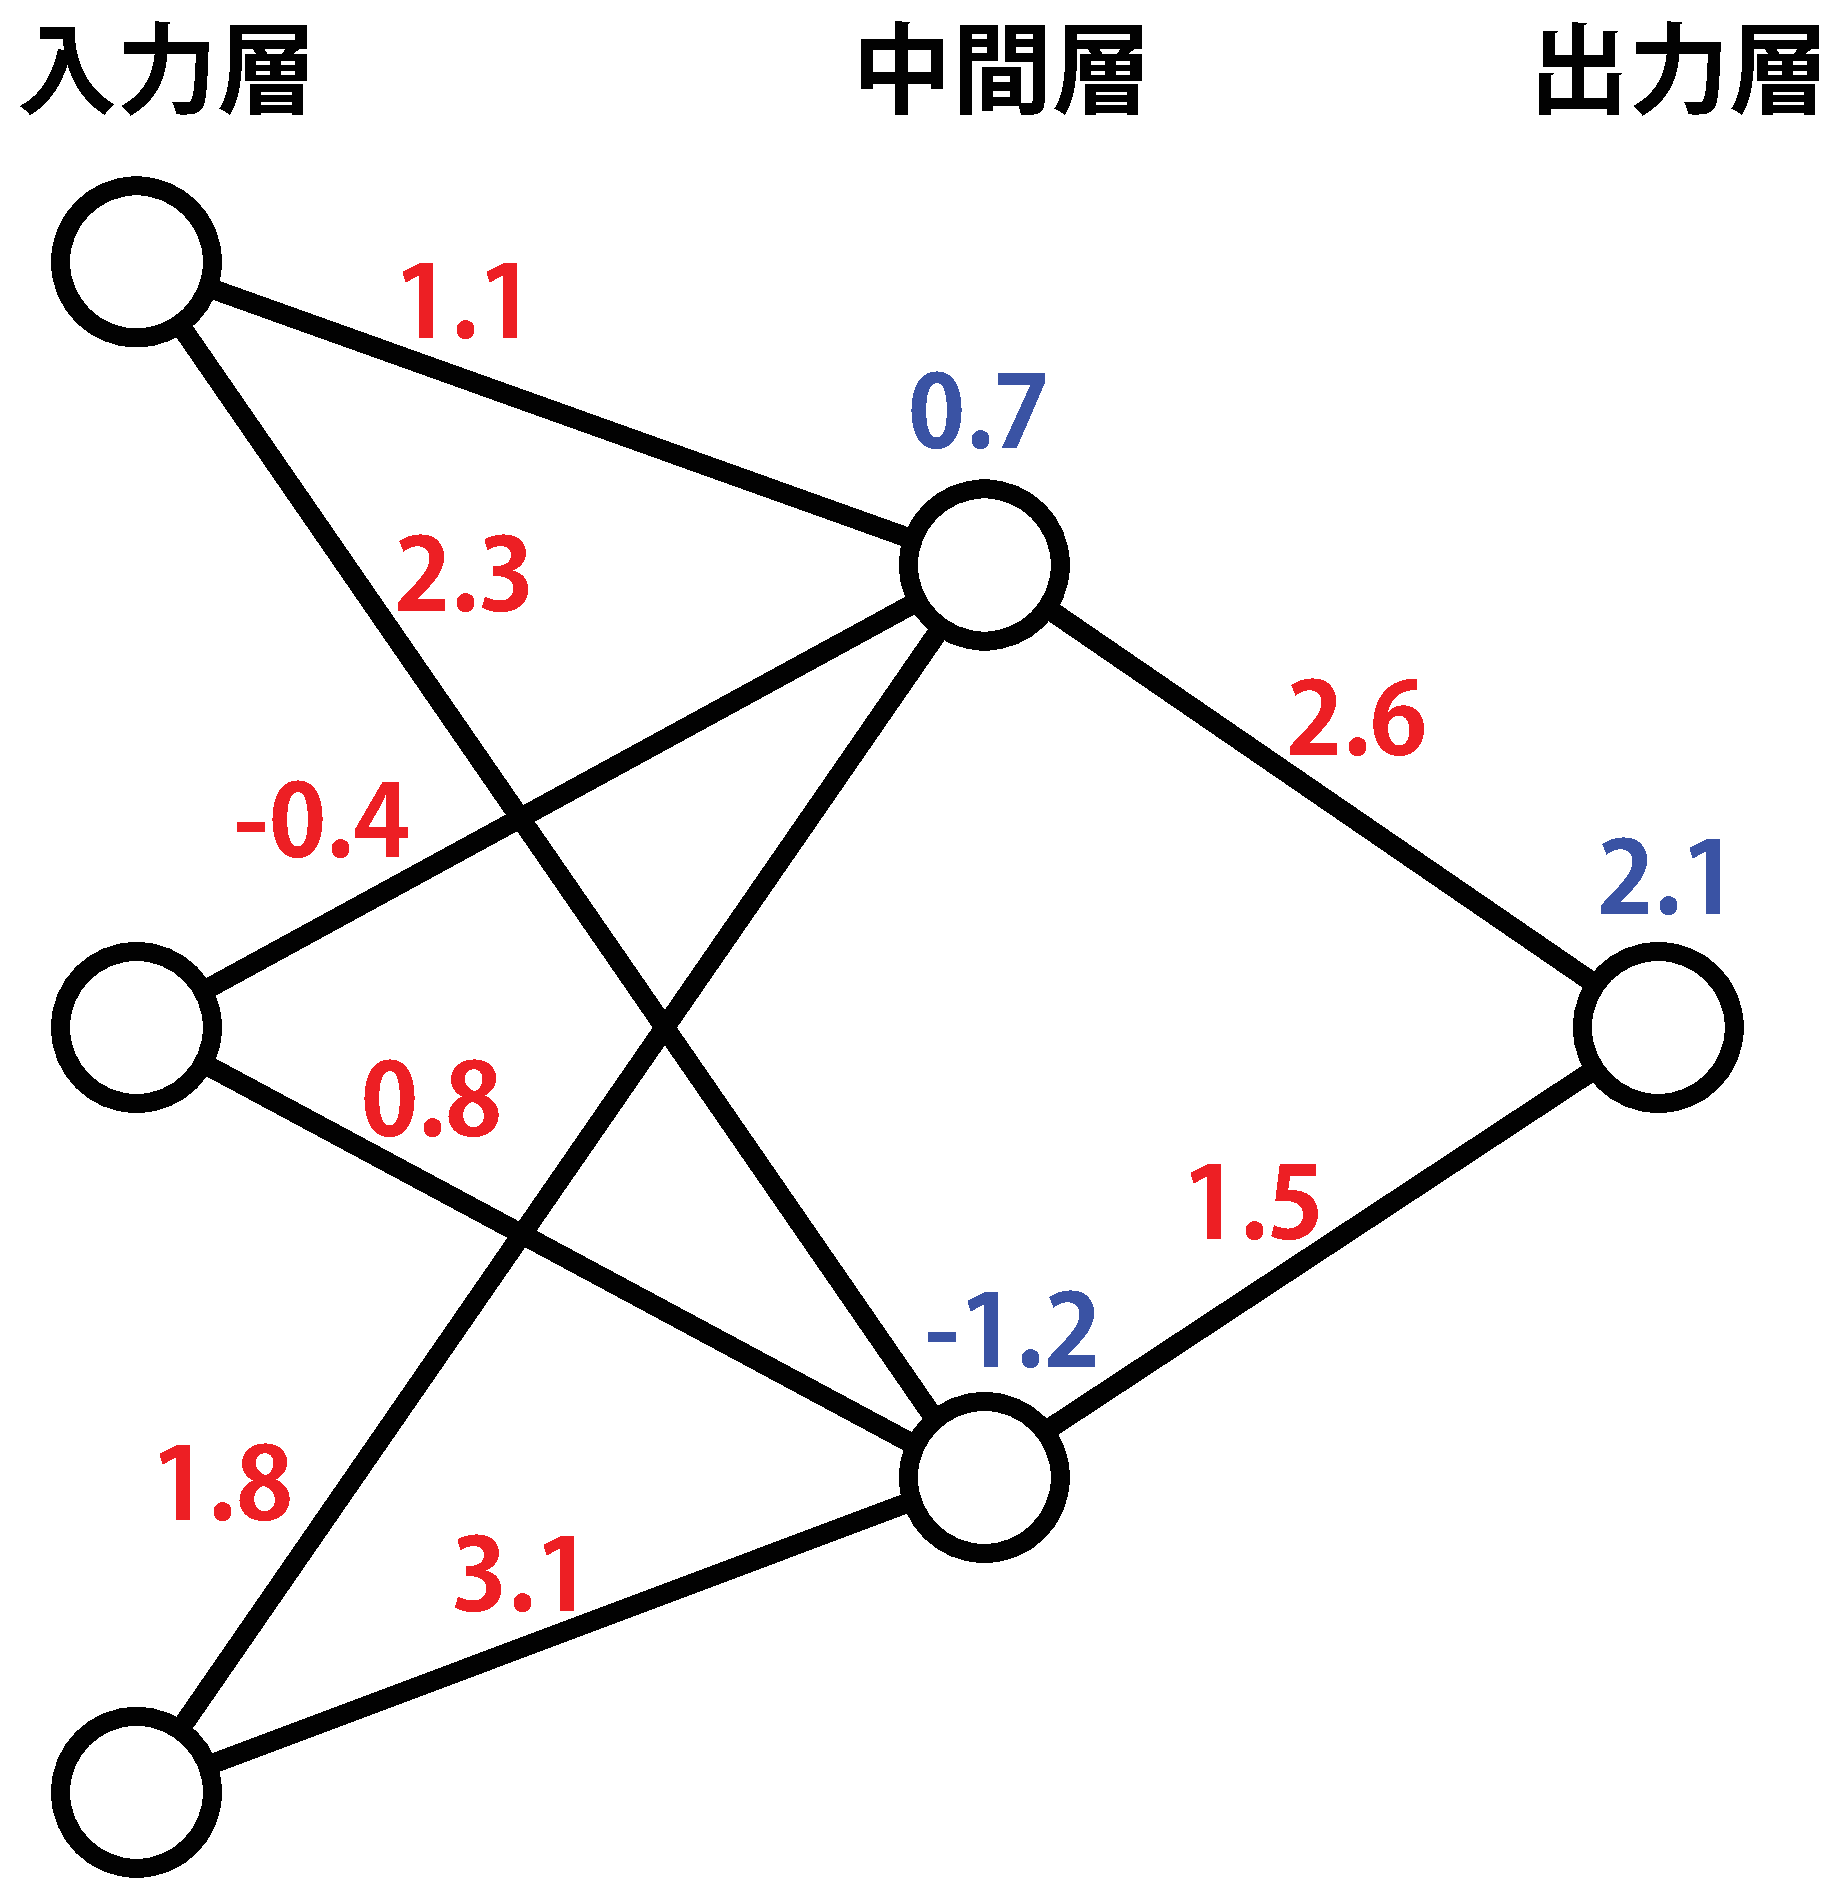
\includegraphics[width = 0.4 \textwidth]{./fig/ANN_sample_jp}
   \caption{ニューラルネットワークの具体例.
   赤色の数値が重み,青色の数値がバイアスを表している.枝はすべて左から右に向いている.}
   \label{fig:sample}
\end{figure}

\paragraph{入力層,隠れ層,出力層.}
人工ニューラルネットワークの多層パーセプトロンモデルを仮定する.このモデルでは,ニューラルネットワークはいくつかの層で構成されている.最初の層は入力層で,入力層は場合によっては特徴ベクトルから数値データを得るため,特徴ベクトルの要素と同じ数のノードがある.次に数値は隠れ層を介して伝播される.隠れ層は1つの層の計算が次の層への入力として用いられる.最後に出力層が入力ベクトルに基づいた予測値を与える.

\figref{sample}では,入力層は3つのノードを持つ.
したがって入力する特徴ベクトルは3次元のものでなければならない.
また1つの隠れ層を有し,この隠れ層は2つのノードを持つ.
そして出力層は1つのノードを持つ.

\paragraph{重み.}
ニューラルネットワークでは,ノード間を接続する枝(有向枝)にはそれぞれ数値が割り当てられ,
その値を重みと呼ぶ.入力層から出力層への値の伝播には,これらの重みに基づく計算が含まれている.

\figref{sample}では,枝の重みは赤によって示される.


\paragraph{バイアス.}
ニューラルネットワークの隠れ層の各ノードにはバイアスと呼ばれる数値が割り当てられている.この数値は重みと共に,入力ベクトルに基づいて出力値を計算する過程で使用される.

\figref{sample}では,ノードのバイアスは青によって示される.

\paragraph{活性化関数.}
活性化関数はニューラルネットワークの各ノードに割り当てられており,
与えられた入力ベクトルから出力値を計算する際に用いられる.
特に各ノードの出力値は,重み付けされた対応する枝の重みと
前の層からのノードの出力の線形結合を入力として与えられた活性化関数の値である.

本プロジェクトでは,隱れ層の各ノードの活性化関数として
Rectified Linear-Unit (ReLU) 関数を限定して用いる.
これは次の モジュール3 (この モジュール2 で学習したニューラルネットワークに基づいた化合物推定)
では,活性化関数が ReLU であることを仮定しているからである. 

\medskip

%ニューラルネットワークは,与えられた入力ベクトルと目標値の組に基づいて
%重みとバイアスの組を計算する.このプロセスは一般に「学習」と呼ばれる.

\invis{
\section{ファイル構成}
パッケージに含まれるファイルとその役割は\tabref{files}の通りである.
\begin{table}[h!]
  \centering
  \caption{モジュール2 のパッケージに含まれるファイルとその役割}
  \label{tab:files}
  \begin{tabular}{lcll}
  \hline
  \bf ファイル名 &\ \ & \multicolumn{2}{l}{\bf 役割}\\
  \hline
  \verb|mol-infer_ANN.py| && \multicolumn{2}{l}{NNを学習するためのPythonスクリプト}\\
  &&\multicolumn{2}{l}{\bf (モジュール3に進むにはこのスクリプトの実行が必要)}\\
  &&\multicolumn{2}{l}{$\bullet$使用する非標準ライブラリ: {\tt numpy, pandas, scikit-learn}}\\
  \hline
  \verb|predict_values.py| && \multicolumn{2}{l}{学習したNNを用いて}\\
  &&\multicolumn{2}{l}{化学的性質の値を推定するための補助的なPythonスクリプト}\\
  &&\multicolumn{2}{l}{(このスクリプトの実行は必ずしも必要ではない)}\\
  &&\multicolumn{2}{l}{$\bullet$使用する非標準ライブラリ: {\tt numpy, pandas}}\\
  \hline
  \multicolumn{4}{l}{\tt Manual\_Module\_2\_Cyclic\_jp.pdf}\\
  \multicolumn{4}{l}{\tt Manual\_Module\_2\_Cyclic\_jp.tex}\\
  %\multicolumn{4}{l}{\tt Manual\_Module\_2\_Cyclic\_improved\_jp.pdf}\\
  %\multicolumn{4}{l}{\tt Manual\_Module\_2\_Cyclic\_improved\_jp.tex}\\
  \multicolumn{4}{l}{\tt fig/ANN\_sample\_jp.eps}\\
  &&\multicolumn{2}{l}{マニュアルのPDF,\LaTeX ソースファイル}\\
  &&\multicolumn{2}{l}{および画像ファイル(日本語版)}\\
  \hline
  \multicolumn{4}{l}{\tt Manual\_Module\_2\_Cyclic\_en.pdf}\\
  \multicolumn{4}{l}{\tt Manual\_Module\_2\_Cyclic\_en.tex}\\
  %\multicolumn{4}{l}{\tt Manual\_Module\_2\_Cyclic\_improved\_en.pdf}\\
  %\multicolumn{4}{l}{\tt Manual\_Module\_2\_Cyclic\_improved\_en.tex}\\
  \multicolumn{4}{l}{\tt fig/ANN\_sample\_en.eps}\\
  &&\multicolumn{2}{l}{マニュアルのPDF,\LaTeX ソースファイル}\\
  &&\multicolumn{2}{l}{および画像ファイル(英語版)}\\
  \hline
  \multicolumn{4}{l}{\bf BP (boiling point; 沸点) に関するデータファイル~\cite{pubchem}}\\
  \multicolumn{2}{l}{\tt data/BP.sdf} & \multicolumn{2}{l}{化合物に関するSDFファイル.モジュール2 では直接取り扱わない}\\
  \multicolumn{2}{l}{\tt data/BP\_fv.csv} & \multicolumn{2}{l}{モジュール1 に{\tt BP.sdf}を入力して生成した特徴ベクトル}\\
  \multicolumn{2}{l}{\tt data/BP\_value.csv} & \multicolumn{2}{l}{化合物のBP値を記したファイル}\\
  \multicolumn{2}{l}{\tt data/BP\_ANN.LOG} & \multicolumn{2}{l}{{\tt BP\_fv.csv, BP\_value.csv}から成るデータセットに対して}\\
  &&\multicolumn{2}{l}{{\tt mol-infer\_ANN.py}を実行し,学習したときのログ出力}\\
  \multicolumn{4}{l}{\tt data/BP\_ANN\_biases.txt} \\
  \multicolumn{4}{l}{\tt data/BP\_ANN\_weights.txt} \\
  &&\multicolumn{2}{l}{学習されたNNにおける各ノードのバイアス,}\\
  &&\multicolumn{2}{l}{および各枝の重み}\\
  \hline
  \end{tabular}
\end{table}

\newpage

\begin{table}[t!]
  \centering
  (\tabref{files}の続き)
  \begin{tabular}{lcll}
  \hline
  \bf ファイル名 &\ \ & \multicolumn{2}{l}{\bf 役割}\\
  \hline
  \multicolumn{4}{l}{\bf HC (heat of combustion; 燃焼熱) に関するデータファイル~\cite{pubchem}}\\
  \multicolumn{2}{l}{\tt data/HC.sdf} & \multicolumn{2}{l}{化合物に関するSDFファイル.モジュール2 では直接取り扱わない}\\
  \multicolumn{2}{l}{\tt data/HC\_fv.csv} & \multicolumn{2}{l}{モジュール1 に{\tt HC.sdf}を入力して生成した特徴ベクトル}\\
  \multicolumn{2}{l}{\tt data/HC\_value.csv} & \multicolumn{2}{l}{化合物のHC値を記したファイル}\\
  \multicolumn{2}{l}{\tt data/HC\_ANN.LOG} & \multicolumn{2}{l}{{\tt HC\_fv.csv, HC\_value.csv}から成るデータセットに対して}\\
  &&\multicolumn{2}{l}{{\tt mol-infer\_ANN.py}を実行し,学習したときのログ出力}\\
  \multicolumn{4}{l}{\tt data/HC\_ANN\_biases.txt} \\
  \multicolumn{4}{l}{\tt data/HC\_ANN\_weights.txt} \\
  &&\multicolumn{2}{l}{学習されたNNにおける各ノードのバイアス,}\\
  &&\multicolumn{2}{l}{および各枝の重み}\\
  \hline
  \multicolumn{4}{l}{\bf KOW (log Kow; オクタノール/水分配係数) に関するデータファイル~\cite{pubchem}}\\
  \multicolumn{2}{l}{\tt data/KOW.sdf} & \multicolumn{2}{l}{化合物に関するSDFファイル.モジュール2 では直接取り扱わない}\\
  \multicolumn{2}{l}{\tt data/KOW\_fv.csv} & \multicolumn{2}{l}{モジュール1 に{\tt KOW.sdf}を入力して生成した特徴ベクトル}\\
  \multicolumn{2}{l}{\tt data/KOW\_value.csv} & \multicolumn{2}{l}{化合物のKOW値を記したファイル}\\
  \multicolumn{2}{l}{\tt data/KOW\_ANN.LOG} & \multicolumn{2}{l}{{\tt KOW\_fv.csv, KOW\_value.csv}から成るデータセットに対して}\\
  &&\multicolumn{2}{l}{{\tt mol-infer\_ANN.py}を実行し,学習したときのログ出力}\\
  \multicolumn{4}{l}{\tt data/KOW\_ANN\_biases.txt} \\
  \multicolumn{4}{l}{\tt data/KOW\_ANN\_weights.txt} \\
  &&\multicolumn{2}{l}{学習されたNNにおける各ノードのバイアス,}\\
  &&\multicolumn{2}{l}{および各枝の重み}\\
  \hline
  \multicolumn{4}{l}{\bf MP (melting point; 融点) に関するデータファイル~\cite{pubchem}}\\
  \multicolumn{2}{l}{\tt data/MP.sdf} & \multicolumn{2}{l}{化合物に関するSDFファイル.モジュール2 では直接取り扱わない}\\
  \multicolumn{2}{l}{\tt data/MP\_fv.csv} & \multicolumn{2}{l}{モジュール1 に{\tt MP.sdf}を入力して生成した特徴ベクトル}\\
  \multicolumn{2}{l}{\tt data/MP\_value.csv} & \multicolumn{2}{l}{化合物のMP値を記したファイル}\\
  \multicolumn{2}{l}{\tt data/MP\_ANN.LOG} & \multicolumn{2}{l}{{\tt MP\_fv.csv, MP\_value.csv}から成るデータセットに対して}\\
  &&\multicolumn{2}{l}{{\tt mol-infer\_ANN.py}を実行し,学習したときのログ出力}\\
  \multicolumn{4}{l}{\tt data/MP\_ANN\_biases.txt} \\
  \multicolumn{4}{l}{\tt data/MP\_ANN\_weights.txt} \\
  &&\multicolumn{2}{l}{学習されたNNにおける各ノードのバイアス,}\\
  &&\multicolumn{2}{l}{および各枝の重み}\\
  \hline
  \end{tabular}

\end{table}
}

%%%%%%%%%%%%%%%%%%%%%%%%%%%%%%%%%%%%%%%%%%%%%%%%%%%%%%%%%%%%
%\clearpage
\section{クイックスタート}
\label{chap:2quick}

\paragraph{ニューラルネットワークの学習.}

次のコマンドを入力すれば,
\verb|instances/BP/BP_desc.csv|を特徴ベクトル,
\verb|instances/BP/BP_values.csv|を化学的性質(この場合はBP,すなわち沸点)の値
とするようなデータセットに対し,
2つの隠れ層を持ち,それぞれの隠れ層における
ノード数を20, 10とするようなニューラルネットワークが学習され,
そのニューラルネットワークにおける各枝の重みは\verb|output_weights.txt|,
各ノードのバイアスは
\verb|output_biases.txt|
にそれぞれ出力される.

\begin{oframed}
{\small
\begin{verbatim}
$ python scikit_chemgraph_learning_lim.py ../instances/BP/BP_desc.csv\
 ../instances/BP/BP_values.txt output 20 10
\end{verbatim}
% \hfill $(\clubsuit)$
}
\end{oframed}

学習されたニューラルネットワークの{\bf 重みおよびバイアスに関するファイルは,モジュール3でも使用}する.


\paragraph{化学的性質の値の推定.}
学習したニューラルネットワークを用いて,
化合物の化学的性質の値を推定することができる.

次のコマンド\footnote{一行目の最後のバックスラッシュ $\backslash$ は,実際に入力するときには改行してはならないことを示す.}を入力すれば,
学習済ニューラルネットワーク(枝の重みは\verb|output_weights.txt|,ノードのバイアスは\verb|output_biases.txt|に保持されている)を用いて,\verb|instances/BP/BP_desc.csv|に記述された特徴ベクトル(に対応する化合物)の化学的性質の値が推定され,その結果は\verb|predicted.txt|に出力される.

\begin{oframed}
  {\small
\begin{verbatim}
$ python predict_values.py output_weights.txt output_biases.txt \
    instances/BP/BP_desc.csv predicted.txt
\end{verbatim}
}
  \end{oframed}

\begin{itemize}
\item 化学的性質の値を推定したい化合物の特徴ベクトルは,モジュール1の特徴ベクトル生成器を用いて生成することができる.
%\item 上のコマンドは,さらに上のコマンド$(\clubsuit)$で\verb|data/BP_fv.csv|を
%  特徴ベクトルとしたデータセットから学習したニューラルネットワークに関する \verb|output_weights.txt|および \verb|output_biases.txt|を用いるものとみなせば,
%  データセット自身の化学的性質の値を推定していることになる.
\item この推定機能は補助的なものに過ぎず,モジュール3以降で使用することはない.
\end{itemize}


\section{プログラムの入出力に関する詳細}
\label{chap:2io}

\subsection{入力}
\subsubsection{特徴ベクトル}
特徴ベクトルは,我々が{\bf FV形式}と呼ぶフォーマットに基づく
csvファイルに記述されている必要がある.
モジュール1の特徴ベクトル生成器は
化合物に関するSDFファイルから
FV形式のcsvファイルを生成するため,
当該生成器を用いて生成されたファイルを用いれば問題はない.

FV形式の記述ルールは\chapref{1io}で述べたとおりである.
\invis{
\begin{oframed}
  {\small
\begin{verbatim}
CID,n,cs,ch,nsH
244,8,6,2,8
307,10,6,4,8
657014,11,7,1,18
16704,9,9,0,10
\end{verbatim}
}
\end{oframed}
\begin{itemize}
\item FV形式では先頭行に記述子の名前をコンマ区切りで記述する.
\item ただし最初の記述子は CID(化合物識別番号)でなければならない.CIDの値が学習に用いられることはない.CIDは識別のためのみに用いられる.
\item 上記の例では,\verb|n|(水素を除く原子の個数),\verb|cs|(コアサイズ),\verb|ch|(コアハイト),\verb|nsH|(水素原子の個数)と四つの記述子が定められている.
\item 二行目以降に,一つの行に一つの化合物のCIDおよび特徴ベクトルを,コンマ区切りで記述する.
  したがって各化合物は,4次元の特徴ベクトルで表されることになる.
\item 化合物がCIDの昇順あるいは降順に並んでいる必要はない.
\end{itemize}
}

\subsubsection{化学的性質の値}
化学的性質の値は,CIDと値を羅列したcsvファイルに記述されなければならない.
\begin{oframed}
  {\small
\begin{verbatim}
CID,a
307,11.2
244,-0.5
657014,98.124
16704,-12.8
117,5.3
\end{verbatim}
}
\end{oframed}
\begin{itemize}
\item {\bf 先頭行は\verb|CID,a|でなければならない.}
\item 二行目以降に,一つの行に一つの化合物のCIDおよび化学的性質の値を
  コンマ区切りで記述する.
\item 化合物がCIDの昇順あるいは降順に並んでいる必要はない.
\end{itemize}
  
\subsection{実行}
\chapref{2quick}で示したとおり,
ニューラルネットワークを学習するには{\tt scikit\_chemgraph\_learning\_lim.py}を用いる.

\subsubsection{引数}
\chapref{2quick}で示したコマンドを再掲する.
\begin{oframed}
  {\small  
\begin{verbatim}
$ python scikit_chemgraph_learning_lim.py ../instances/BP/BP_desc.csv\
 ../instances/BP/BP_values.txt output 20 10
\end{verbatim}
%\verb|$ python mol-infer_ANN.py data/BP_fv.csv data/BP_value.csv output 20 10|
}
\end{oframed}
各引数には以下を指定する.
\begin{itemize}
\item 第1引数: 特徴ベクトルに関するcsvファイル
\item 第2引数: 化学的性質の値に関するcsvファイル
\item 第3引数: 学習されたニューラルネットワークの重み・バイアスを書き込むファイルの名前
\item 第4引数以降: 隠れ層(中間層)のノードの個数
\end{itemize}

\invis{
引数を与えずに実行すれば(もしくは引数が適切に与えられなかった場合),
引数に関する説明が英語で出力される.
\begin{oframed}
  {\small
\begin{verbatim}
$ python mol-infer_ANN.py 
\end{verbatim}
  }
  \end{oframed}
}

引数が適切に与えられると,ニューラルネットワークの学習が始まる.

5分割交差検定が行われ,試験集合に対して最も高い決定係数 (${\rm R}^2$値) を
実現するニューラルネットワークが採用され,
その重みとバイアスが,ファイルに出力される.
上記のコマンドの場合,そのファイルの名前は第3引数で指定された\verb|output|に基づく,
\begin{itemize}
\item \verb|output_weights.txt|(重み)
\item \verb|output_biases.txt|(バイアス)
\end{itemize}
である.これら出力されたファイルは,モジュール3 の実行に必要となる.


\paragraph{データセットに関する注意.}
データセットは,
\begin{itemize}
\item 特徴ベクトルに関するcsvファイル,および
\item 化学的性質の値に関するcsvファイル
\end{itemize}
の二つのファイルから構成されるが,
CID は前者ファイルに記されたものすべて,かつそれのみが計算の対象となる.
したがって,
\begin{center}
  {\bf 前者ファイルに記されたCIDは,
  すべて後者ファイルに記されていなければならない.}
\end{center}
しかし逆は成り立たなくともよい.
つまり,化学的性質の値に関するcsvファイルには,
特徴ベクトルのcsvファイルに記されていない,
「余計な」CIDに関する値が記されていても構わない.
そのような値は無視される.

\subsubsection{ハイパーパラメータの調整}
ニューラルネットワークの学習は{\tt scikit-learn}ライブラリ\footnote{\url{https://scikit-learn.org/stable/}}
における{\tt MLPRegressor}を用いて行われる.
\verb|scikit_chemgraph_learning_lim.py|の
135行目以降で\verb|MLPRegressor|インスタンスの初期化が行われるが,
ハイパーパラメータの調整はここで行うことができる.
一部のパラメータを以下のように設定している.
\begin{itemize}
\item \verb|activation|: \verb|'relu'| {\color{red}{\bf 注意:} 学習されたニューラルネットワークを モジュール3 以降で用いるには, \verb|'relu'| (ReLU関数) でなければならない.}
\item \verb|alpha|: $10^{-5}$
\item \verb|early_stopping|: \verb|False|
\item \verb|hidden_layer_sizes|: 実行時に引数で指定した個数に基づく
\item \verb|max_iter|: $10^{10}$
\item \verb|random_state|: 1
\item \verb|solver|: \verb|'adam'|
\end{itemize}

\subsection{出力}
ふたたび以下のコマンドを取り上げ,
その実行によって得られる出力について説明する.
\begin{oframed}
  {\small
    \begin{verbatim}
$ python scikit_chemgraph_learning_lim.py ../instances/BP/BP_desc.csv\
 ../instances/BP/BP_values.txt output 20 10
\end{verbatim}
}
\end{oframed}

\subsubsection{標準出力}
上記コマンドを実行すると端末(標準出力)に計算過程が出力される.
この出力例がパッケージ内のファイル\verb|instances/BP/BP_ANN.LOG|に記されている.
\invis{
\begin{oframed}
  {\small
\begin{verbatim}
src/preparation/BP_fv.csv contains 181 vectors for 107 (=CID+106) features.
src/preparation/BP_value.csv contains 230 target values.
n range = [5,30]
a range = [31.5,470.0]
#instances = 181
#features = 106

D1: train 144, test 37
training time: 3.187196731567383
R2 score train = 0.9935319077425955
R2 score test = 0.7855694851759929
R2 score all = 0.9599908495442584
MAE score train = 3.8570127089010384
MAE score test = 19.756408746147212
MAE score all = 7.10716548999556

D2: train 145, test 36
training time: 5.0139079093933105
R2 score train = 0.9930416804444452
R2 score test = 0.6390572625074291
R2 score all = 0.9339056805642507
MAE score train = 3.7281172621746888
MAE score test = 27.996544836634186
MAE score all = 8.554986834995363

D3: train 145, test 36
training time: 4.264358758926392
R2 score train = 0.9961346879653636
R2 score test = 0.8566979846124056
R2 score all = 0.9637772344809027
MAE score train = 2.870368503215682
MAE score test = 22.925217956024927
MAE score all = 6.8591783391335435

D4: train 145, test 36
training time: 2.9935202598571777
R2 score train = 0.9909067339023991
R2 score test = 0.8390994594153819
R2 score all = 0.9669036994338265
MAE score train = 4.470398694611737
MAE score test = 18.691072072382227
MAE score all = 7.298819918919681

D5: train 145, test 36
training time: 4.9648661613464355
R2 score train = 0.9946933391220482
R2 score test = 0.8479544758088942
R2 score all = 0.9574271159388575
MAE score train = 3.352287445970431
MAE score test = 21.80973582058148
MAE score all = 7.023382150312958
0.9935319077425955 0.7855694851759929 0.9599908495442584 3.187196731567383
0.9930416804444452 0.6390572625074291 0.9339056805642507 5.0139079093933105
0.9961346879653636 0.8566979846124056 0.9637772344809027 4.264358758926392
0.9909067339023991 0.8390994594153819 0.9669036994338265 2.9935202598571777
0.9946933391220482 0.8479544758088942 0.9574271159388575 4.9648661613464355
Average time = 4.08476996421814
Average R2 test score = 0.7936757335040208
Average MAE test score = 22.235795886354005
  \end{verbatim}        
}
\end{oframed}

\begin{itemize}
\item  冒頭で特徴ベクトルの個数,特徴数が出力される.また水素を除く原子数(特徴\verb|n|)の最小値と最大値 (\verb|n range|,上の例では5と30),および化学的性質(この場合はBP; 沸点)の値の
最小値と最大値(\verb|a range|,上の例では31.5と470.0)が出力される.
\item 続いて5分割交差検定における5回の学習の概要が出力される.
\item 最後に平均計算時間,(試験集合に対する)平均R$^2$値,
(試験集合に対する)平均MAE値が出力される.
\item 上記の例では,3回目の学習で得られたニューラルネットワークが
最も高い(試験集合に対する)R$^2$値を達成しているので(0.856697$\dots$),
当該ニューラルネットワークにおける枝重みが\verb|output_weights.txt|,
ノードのバイアスが\verb|output_biases.txt|に出力される.
\item なおこれらファイルのコピーを,それぞれ
\verb|data/BP_ANN_weights.txt|,\verb|data/BP_ANN_biases.txt|
として同封している.
\end{itemize}
}

\subsubsection{枝の重み}
\verb|scikit_chemgraph_learning_lim.py|が出力する枝重みファイルの書式について説明する.

簡単のため,\figref{sample}に示したニューラルネットワークが学習されたとする.
このニューラルネットワークの枝重みは以下のようにファイルに出力される.

\begin{oframed}
{\small
\begin{verbatim}
3 2 1
1.1 2.3
-0.4 0.8
1.8 3.1
2.6
1.5
\end{verbatim}
}
\end{oframed}
\begin{itemize}
\item 最初の行はニューラルネットワークの構造,つまり入力層のノード数,各隠れ層のノード数,最後に出力層のノード数である.
\item 2行目以降は枝重みの値である.各行は1つのノードから出る枝重みの値を示す.
\end{itemize}


\subsubsection{ノードのバイアス}
同じく,\verb|scikit_chemgraph_learning_lim.py|が出力するノードの
バイアスに関するファイルの書式について説明する.

やはり簡単のため,\figref{sample}に示したニューラルネットワークが学習されたとする.
このニューラルネットワークのノードのバイアスは以下のようにファイルに出力される.

\begin{oframed}
{\small
\begin{verbatim}
0.7
-1.2
2.1
\end{verbatim}
}
\end{oframed}
1行につき1つのノードのバイアスの値が示されている.
入力層のノードにはバイアスの値がないことに注意せよ.

%%%%%%%%%%%%%%%%%%%%%%%%%%%%%%%%%%%%%%%%%%%%%%%%%%%%%%%%%%%%
\chapter{モジュール3: MILPを用いた環構造化学グラフの推定}
\label{chap:3Intro}

この章では,学習済み人工ニューラルネットワーク (ANN) の重みとバイアスと\target 値を与えられた時に,
デスクリプタ (記述子) のベクトルを推定できる混合整数線形計画法 (Mixed Integer Linear Programming; MILP) の使い方を説明する.

MILPを定義する機能はPythonで実装されていて,
COIN-ORパッケージのPuLPモデリングモジュール~\cite{PuLP1,PuLP2,PuLP3,PuLP4}を使用する.

\invis{
まず,この冊子に添付されているファイルの一覧を示す.

\begin{itemize}

\item フォルダ {\tt source\_code}\\
  与えられたANNに対し,
  環式化学グラフの特徴ベクトルを推定するためのMILPを実装した
  四つのpythonスクリプトと,
  MILP定式化における各デスクリプタの最小値と最大値を含むファイルを含むフォルダ.

\begin{itemize}

\item {\tt ann\_inverter.py}\\
ANNの逆問題に対する定式化したMILPを実装したスクリプト~\cite{AN19}.

\item {\tt cyclic\_graphs\_MILP\_ec\_id.py}\\
変数を初期化し,規定のトポロジ構造~\cite{cyclic_BH_arxiv}を持つ環式化学グラフを推定するための定式化したMILPの制約を用意する関数を含むPythonスクリプト.

\item {\tt infer\_cyclic\_graphs\_ec\_id.py}\\
データを用意し,指定の入力データに対して定式化したMILPを実行するPythonスクリプト.
このスクリプトの使用に関する詳細は,第\ref{chap:Exp}節に記載されている.

\item {\tt read\_instance\_BH\_cyclic.py}\\
与えられたテキストファイルからトポロジカル仕様を読み取るために必要な関数を含むPythonスクリプト.

\item フォルダ {\tt topological\_description}\\
論文~\cite{cyclic_BH_arxiv}で詳述されている化学仕様をそれぞれ提供する六つのテキストファイルを含むフォルダ.
%
\begin{itemize}
 \item {\tt instance\_a.txt}
 \item {\tt instance\_b1.txt}
 \item {\tt instance\_b2.txt}
 \item {\tt instance\_b3.txt}
 \item {\tt instance\_b4.txt}
 \item {\tt instance\_c.txt}
 \item {\tt instance\_d.txt}
\end{itemize}

\item フォルダ {\tt ANN}\\
沸点(Bp),融点(Mp),およびオクタノール/水分配係数(Kow)
の三つの\target 特性の学習済み人工ニューラルネットワーク(ANN)に関する情報を含むフォルダ.
上記の三つの各特性${\tt property}\in \{{\tt BP, MP, KOW}\}$ について三つのファイルが提供される.
%
\begin{itemize}
\item {\tt property\_desc.csv}\\
ANNの学習で使用されるデスクリプタを含むコンマ区切り形式のファイル.

\item {\tt property\_biases.txt}\\
学習済みANNのバイアスの値を含むファイル.

\item {\tt property\_weights.txt}\\
学習済みANNの重みの値を含むファイル.
\end{itemize}
%
各ファイルのデータ形式は第\ref{chap:InOut}節で説明されており,実際の例は第\ref{chap:Exp}節で説明されてる.

% \item {\tt fv4\_cyclic\_stdout.cpp}\\
% SDF形式で保存された化学グラフの特徴ベクトルを計算するC ++プログラム.
% このプログラムの入力と出力は,MILPの解として推定されるグラフのデスクリプタ値
% を検証するためにPythonスクリプト{\tt infer\_cyclic\_graphs\_ec\_id.py}
% で動作するようにカスタマイズされている(解が存在する場合).
% このソースファイルは,{\tt fv}という名前の実行ファイルにコンパイルする必要がある.
% 
% \item {\tt fv}\\
% 上記のC ++プログラムの実行可能なバイナリファイル.
% この実行可能ファイルは,オペレーティングシステム
% Linux Mint 18.3を実行しているPC上で{\tt gcc}バージョン5.4.0によってコンパイルされている.
%
\end{itemize}
\end{itemize}
}

この章は次のように構成されている.
第\ref{chap:Pre}節では使用される用語と表記法を説明する.
%
第\ref{chap:InOut}節はプログラムの入力データと出力データを説明し,
第\ref{chap:Exp}節は入力データと計算結果の具体例を示す.

% \newpage

\section{用語と表記法}
\label{chap:Pre}
%
この節では,用語と表記法について説明する.

\begin{itemize}

\item {\bf 特徴ベクトル}\\
%
特徴ベクトルは,デスクリプタと呼ばれる特定のパラメータの数値を格納する.
本研究では,非水素原子の数,ある程度の頂点の数など,グラフ理論のデスクリプタを選択する.

\item {\bf 人工ニューラルネットワーク - ANN}\\
%
人工ニューラルネットワークは,機械学習の方法の一つである.
入力の特徴ベクトルと出力の\target データのペア間の相関関数を構築する方法を提供する.


\item {\bf 入力層, 中間層, 出力層}\\
%
順伝播型ニューラルネットワークの多層パーセプトロンモデルを扱う.
これらのニューラルネットワークは、いくつかの層で構成されている.
最初に入力層があり,各ニューロンは特徴ベクトルの一つの値を入力として受け取る.
次に隠れ層がある.ここでは,入力層からの値が順伝播的に伝播され,一つの層の各ノードが次の層の全てのノードに接続される.
最後に,出力は出力層で与えられる.
単一の\target 値の予測を扱うため,出力層は単一のノードで構成されていると仮定する.

\item {\bf 重み}\\
%
ANN内の二つのノードを接続する各辺には,重みと呼ばれる実数値が割り当てられる.
ANNの学習プロセスの一部で,既知の特徴ベクトルと\target 値のペアに基づいて,それぞれの重みの値を決定する.

\item {\bf バイアス}\\
入力層のノードを除くANNの各ノードには,バイアスと呼ばれる実数値が割り当てられる.バイアスは辺の重みと同様に,学習プロセスを通じて決定される.


\item {\bf 活性化関数}\\
%
ANNでは,各ノードは入力の活性化関数と呼ばれる関数として出力を生成する.
各ノードには,活性化関数としてRectified Linear-Unit(ReLU)関数があると仮定する.これはANNの逆問題のMILP定式化~\cite{AN19}で正確に表すことができる.
%https://scikit-learn.org/stable/modules/generated/sklearn.neural\_network.MLPRegressor.html

\item {\bf 混合整数計画問題(MILP)}\\
%
すべての制約が線形式として与えられ,
いくつかの決定変数が整数値のみを取る必要がある数理計画問題の一種.
MILPの標準的な文献として,\cite{LP}を挙げておく. 

\item {\bf グラフ}\\
頂点の有限集合とエッジの有限集合で構成される抽象的な組合せ構造.ここで各辺は頂点のペアである.
無向グラフを扱う.すなわち,辺が順序付けられていない頂点のペアになっているグラフを扱う.
グラフ理論の初等的な内容に関しては様々な文献 (たとえば~\cite{graph}など) が知られている.

\end{itemize}

% \newpage

\section{プログラムの入力と出力}
\label{chap:InOut}

この節では,プログラムの入力と出力の形式について説明する.
第\ref{chap:section3_1}節ではプログラムの入力形式の例を示し,
第\ref{chap:section3_2}節では具体的な計算例を示す.
次に,第\ref{chap:section3_3}節ではプログラムの出力形式の例を示し,
第\ref{chap:section3_4}節では具体的な計算例を示す.


\subsection{プログラムの入力}
\label{chap:section3_1}

この節では、プログラムへの入力について説明する.
最初の入力には、以下を含む三つのテキストファイルが必要となる. \\
~~~~- CSV形式のデスクリプタ名, \\
~~~~- テキスト形式の学習済みANNの重みと\\
~~~~- テキスト形式の学習済みANNのバイアス. \\

プログラム実行のコマンドラインパラメータとして用いる共通の接頭辞が {\tt TT}の場合,学習済みANNのディスクリプタ名,重み,バイアスが格納されたファイルはそれぞれ {\tt TT\_desc.csv},{\tt TT\_weights.txt}, {\tt TT\_biases.txt}というファイル名で保存されていなければならない.

%
次に,学習済みANNに基づいて化学グラフを推定するための\target 値を指定する.
その次は,\cite{cyclic_BH_arxiv}で説明されているように、テキストファイルで指定された化学仕様と、第\ref{chap:section3_4}節で説明されている出力ファイルのファイル名の接頭辞を指定する.

最後に,使用するMILPソルバープログラムを選択する.以下から選択できる. \\
~~~~- 1: CPLEX(商用MILPソルバー) \cite{cplex}. \\
ファイル{\tt infer\_acyclic\_graphs.py}のパラメータ{\tt CPLEX\_PATH}は、CPLEXプログラム実行可能ファイルの正しいパスに設定する必要があることに注意せよ.\\
~~~~- 2: CBC(無償のオープンソースMILPソルバー).Python用のPuLPパッケージ\cite{PuLP1}に付属している.



\subsection{入力データ形式}
\label{chap:section3_2}

この節では,プログラムの実際の入力例を示す.
特に,第\ref{chap:section3_1}節で述べた三つの入力ファイルの具体例を示す.

このプログラムの目的は,与えられた学習済みANNから所望の出力を生成する特徴ベクトルを計算することである.
図\ref{fig:sample}は学習済みANNの例を示す.

\invis{
\begin{figure}[H]
  \centering
   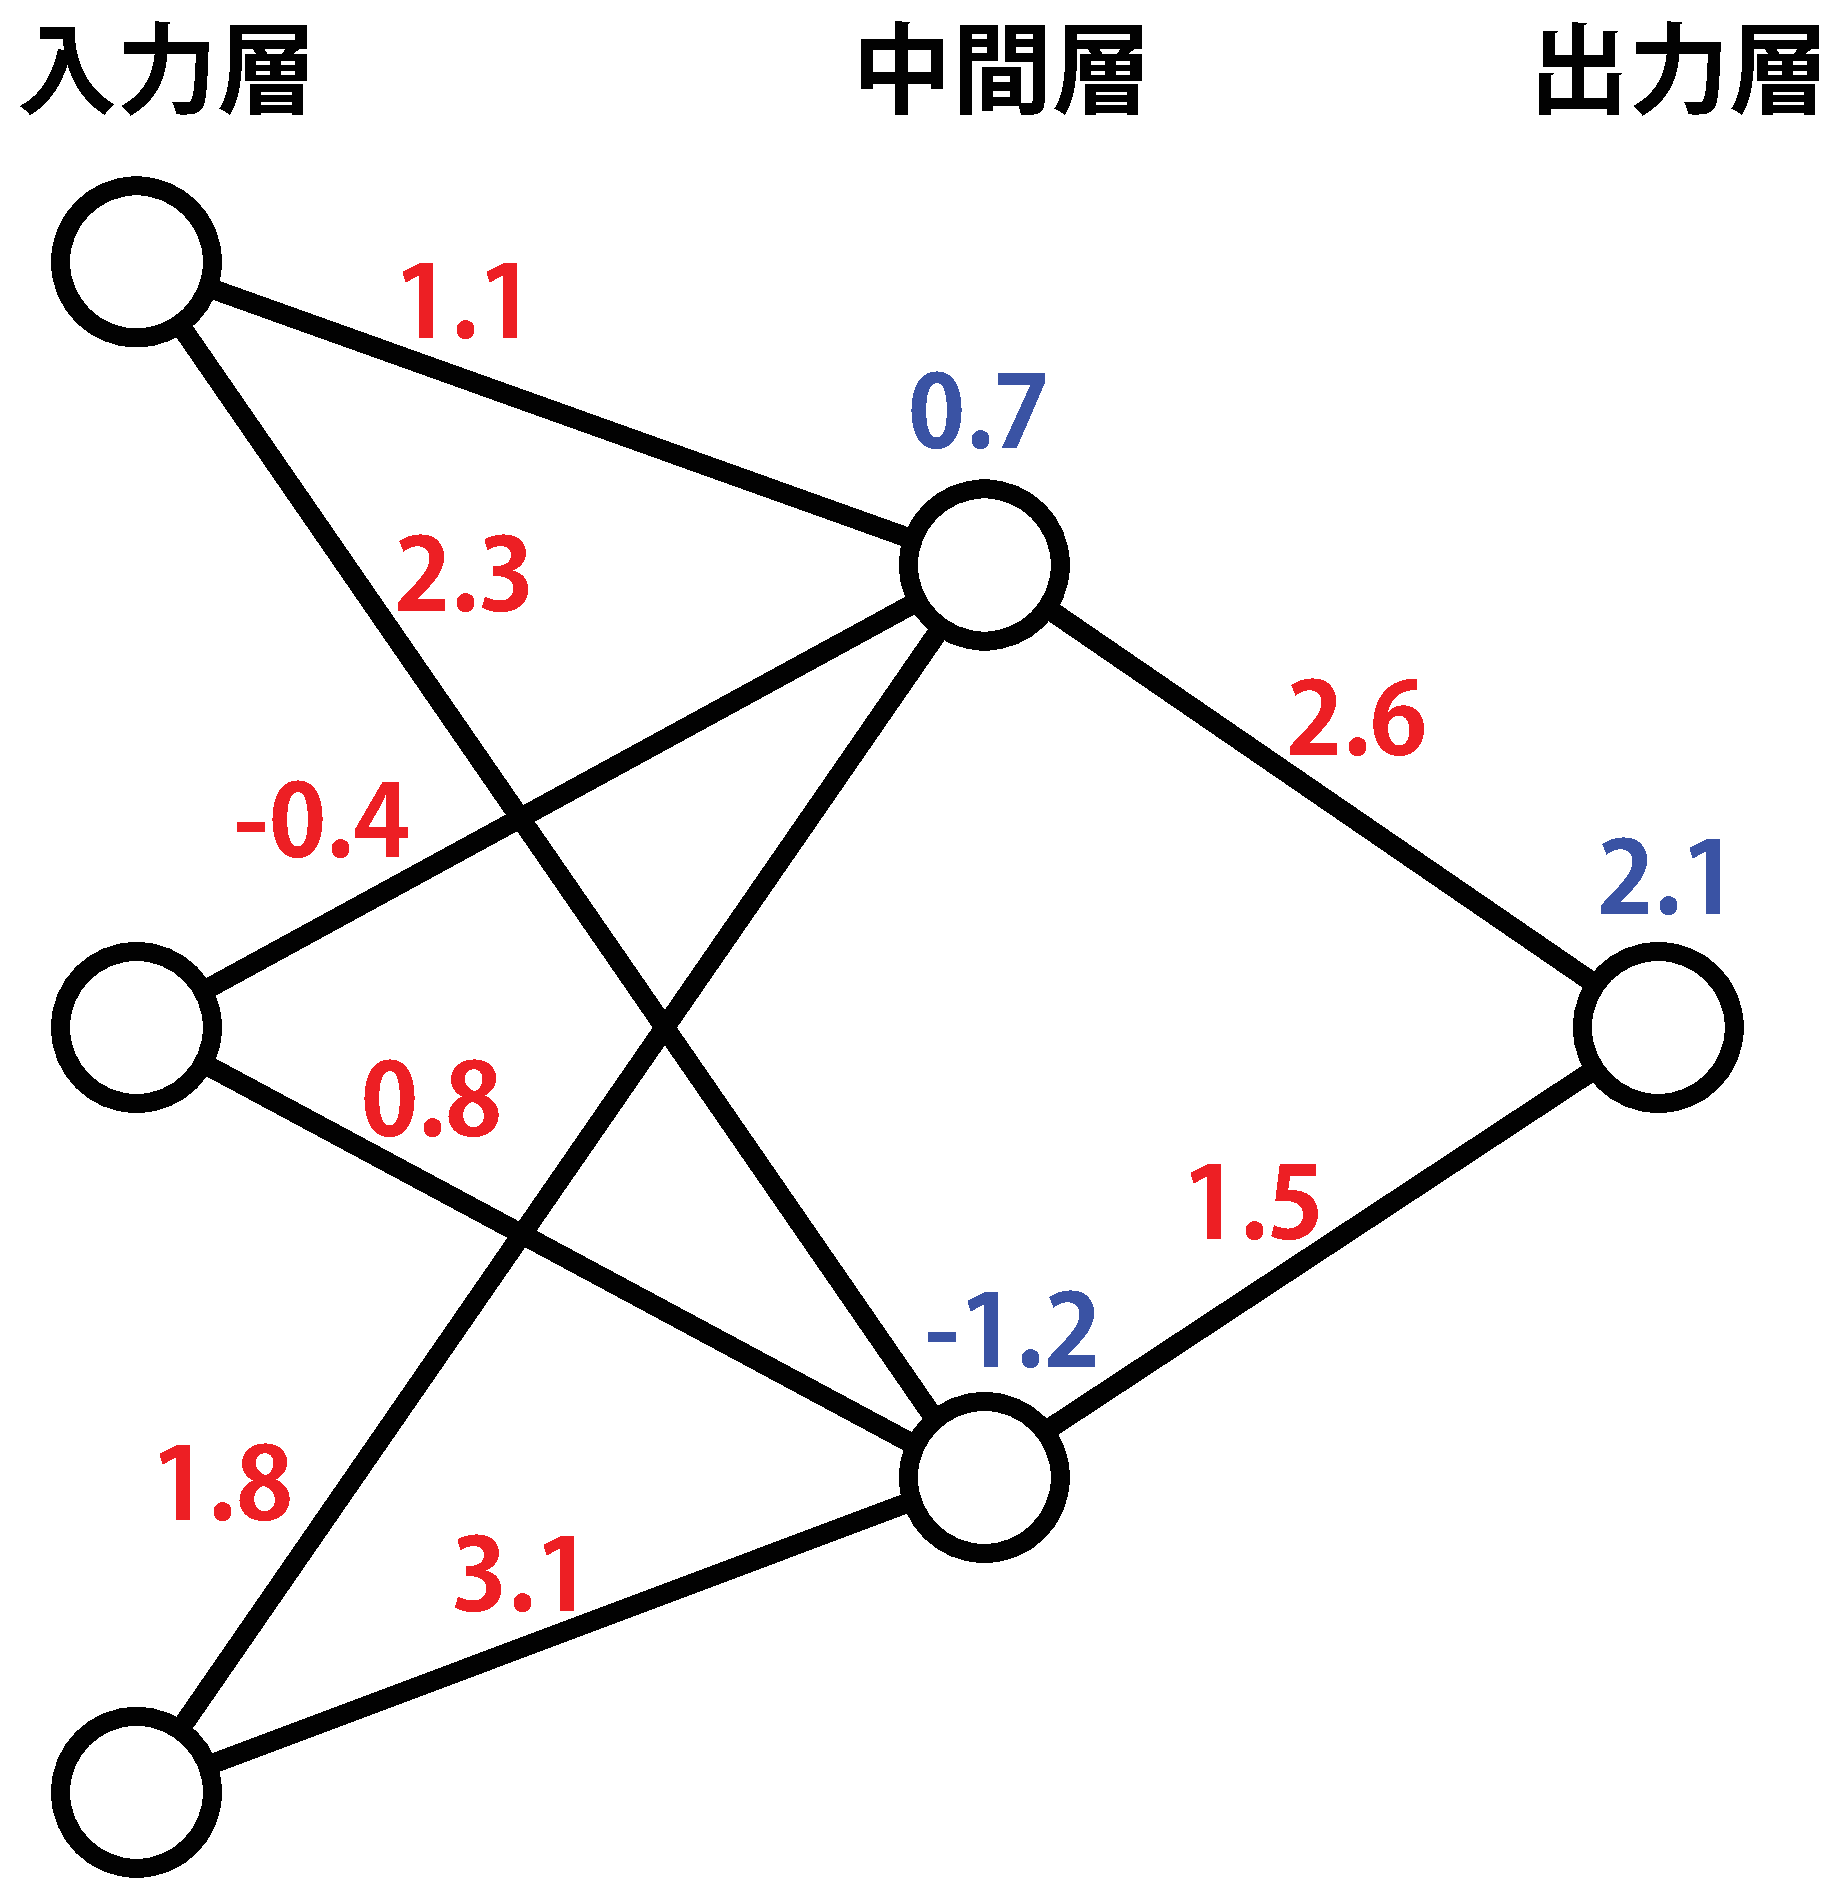
\includegraphics[width=0.5\textwidth]{./fig/ANN_sample_jp}
   \caption{学習済みANNの例.赤い数字はANNの重みを示し,青い数字はバイアスを示す.}
   \label{fig:sample}
\end{figure}
}

学習済みANNの重みとバイアスの情報はそれぞれ二つのテキストファイルに書き込まれる.
まず,重みの情報を含むテキストファイルの構造を示す.
このテキストファイルの最初の行には,ANNのアーキテクチャに関する情報(各レイヤーのノードの数)が書き込まれる.
2行目以降は、ANNの重みが書き込まれる.
各行は,ANNの1つのノードに接続する辺の重みが書き込まれており,最初は入力層のノードの重み,次に隠れ層のノードの重みを表している.
以下に,図\ref{fig:sample}に示されてるANNのテキストファイルの例を示す.

\bigskip

\begin{oframed}
{\bf 重みのデータ形式}\\\\
%\bigskip\bigskip
3 2 1\\
1.1 2.3\\
-0.4 0.8\\
1.8 3.1\\
2.6\\
1.5\\
\end{oframed}

\bigskip


次はANNのバイアスのテキストファイルである.
Fig.~\ref{fig:sample}のバイアスを以下に示す.

\bigskip

\begin{oframed}
{\bf バイアスのデータ形式}\\\\
%\bigskip\bigskip
0.7\\
-1.2\\
2.1\\
\end{oframed}

\bigskip

最後に, 特徴ベクトルのデータが含まれたテキストファイルの形式について説明する.
このファイルの最初の行には,特徴ベクトルで使用されるデスクリプタの名前が書き込まれている.
2行目以降は,トレーニングデータセット内の各化学グラフのデスクリプタの数値が書き込まれている.
一つの化学グラフ毎に1行書き込まれる.
例えば,{\tt ANN}フォルダの{\tt TT\_desc.csv}を確認せよ.
ここで,${\tt TT}\in \{{\tt BP, MP, KOW}\}$である.



\subsection{プログラムの出力}
\label{chap:section3_3}

この節では,プログラムの出力について説明する.
与えられた学習済みANNの予測として与えられた\target 値となるような特徴ベクトルを持つ非環式化合グラフが存在する場合,プログラムは特徴ベクトルを出力する.
そのような化学グラフが存在しない場合,存在しないと出力する.
次の節では,プログラムの出力について説明する.


\subsection{出力データ形式}
\label{chap:section3_4}

この節では,パソコン上で得られたプログラムの出力データについて説明する.
プログラムを実行すると,ターミナルに表示される標準エラーストリームにいくつかのメッセージが出力される.
MILPソルバーが計算を完了すると,計算のステータスがターミナルに表示される.

\bigskip

\begin{oframed}
{\bf ターミナル上の出力結果のデータ形式}\\\\
%\bigskip\bigskip
\begin{tabular}{l l}
 Initializing Time: 0.529                &         \# {\tt stderr}への書き込み \\
Start Solving Using CPLEX...      &       \# {\tt stderr}への書き込み \\
Status: Feasible 				&       \# 解のステータス \\
MILP y*: 223.856 				&      \# MILPで計算された\target 値  \\
ANN propagated y*: 223.856     &      \# 学習済みANNによって計算された\target 値  \\
Solving Time: 52.534                     &      \# MILPソルバーの所要時間 \\
\end{tabular}



\end{oframed}

最後に,実行可能解が存在する場合、プログラムは二つのテキストファイルを出力する.
プログラムは出力ファイルのファイル名を入力の一部として要求することに注意せよ.
出力ファイル名として与えられたパラメータが{\tt filename}であると仮定する.
結果として得られる二つのテキストファイルのファイル名を以下に示す. \\
- {\tt filename.sdf}\\
- {\tt filename\_partition.sdf}. 

\noindent
{\tt filename.sdf}は推定された化学グラフの情報がSDF(Structure Data File)形式で書き込まれている.
詳細については,公式ドキュメント(英語)を参照せよ. \\
\url{http://help.accelrysonline.com/ulm/onelab/1.0/content/ulm_pdfs/direct/reference/}\\
\phantom{\url{http://}}\url{ctfileformats2016.pdf}\\

\noindent
{\tt filename\_partition.sdf}には,\cite{cyclic_BH_arxiv}で説明されているように,{\tt filename.sdf}から非巡回部分グラフへの閉路グラフの分解が含まれている.

\section{プログラムの実行と計算例}
\label{chap:Exp}

この節では,プログラムを実行する方法と具体的な計算例について説明する.
以下は,{\tt infer\_cyclic\_graphs\_ec\_id.py}を実行する例である.

\subsection{プログラムの実行}
\label{chap:Exp_1}

%まず第\ref{chap:Intro}節で説明されているように,ターミナルが{\tt source\_code}フォルダの場所に正しく移動されていることを確認する.



\noindent
{\tt 
 python  infer\_cyclic\_graphs\_ec\_id.py 
trained\_ann\_filename\_prefix
target\_value \\
 \phantom{python }
 chemical\_specification
output\_file\_name
solver\_type
 }\\

例として\target 特性の融点を使用する.ファイル名の接頭辞がMPとなる学習済みANN、\target 値を220、化学仕様のためのファイルを{\tt instance\_1.txt},MILPソルバー(パラメータ値は1)をCPLEX\cite{cplex}とする.

{\tt 
 python infer\_cyclic\_graphs\_ec\_id.py 
ANN/MP
220 \\
 \phantom{python }
chemical\_specification/instance\_a.txt
result
1
 }\\


上記のコマンドを実行すると,ターミナルプロンプトに次のテキストが表示される.

\bigskip

\begin{oframed}
{\bf ターミナル上の出力}\\\\
%\bigskip\bigskip
 Initializing Time: 0.529  \\
Start Solving Using CPLEX...\\
Status: Feasible 		\\
MILP y*: 223.856 		\\
ANN propagated y*: 223.856 \\
Solving Time: 52.534       
\end{oframed}

出力ファイル{\tt result.sdf}および{\tt result\_partition.txt}の内容を以下に示す.

\bigskip

\begin{oframed}
{\bf File {\tt result.sdf}}\\\\
\begin{verbatim}
 1
MILP_cyclic

 48 51  0  0  0  0  0  0  0  0999 V2000 
    0.0000    0.0000    0.0000 C   0  0  0  0  0  0  0  0  0  0  0  0
    0.0000    0.0000    0.0000 C   0  0  0  0  0  0  0  0  0  0  0  0
    0.0000    0.0000    0.0000 C   0  0  0  0  0  0  0  0  0  0  0  0
    0.0000    0.0000    0.0000 O   0  0  0  0  0  0  0  0  0  0  0  0
    0.0000    0.0000    0.0000 C   0  0  0  0  0  0  0  0  0  0  0  0
    0.0000    0.0000    0.0000 C   0  0  0  0  0  0  0  0  0  0  0  0
    0.0000    0.0000    0.0000 C   0  0  0  0  0  0  0  0  0  0  0  0
    0.0000    0.0000    0.0000 O   0  0  0  0  0  0  0  0  0  0  0  0
    0.0000    0.0000    0.0000 C   0  0  0  0  0  0  0  0  0  0  0  0
    0.0000    0.0000    0.0000 C   0  0  0  0  0  0  0  0  0  0  0  0
    0.0000    0.0000    0.0000 C   0  0  0  0  0  0  0  0  0  0  0  0
    0.0000    0.0000    0.0000 C   0  0  0  0  0  0  0  0  0  0  0  0
    0.0000    0.0000    0.0000 N   0  0  0  0  0  0  0  0  0  0  0  0
    0.0000    0.0000    0.0000 C   0  0  0  0  0  0  0  0  0  0  0  0
    0.0000    0.0000    0.0000 C   0  0  0  0  0  0  0  0  0  0  0  0
    0.0000    0.0000    0.0000 O   0  0  0  0  0  0  0  0  0  0  0  0
    0.0000    0.0000    0.0000 C   0  0  0  0  0  0  0  0  0  0  0  0
    0.0000    0.0000    0.0000 N   0  0  0  0  0  0  0  0  0  0  0  0
    0.0000    0.0000    0.0000 C   0  0  0  0  0  0  0  0  0  0  0  0
    0.0000    0.0000    0.0000 C   0  0  0  0  0  0  0  0  0  0  0  0
    0.0000    0.0000    0.0000 C   0  0  0  0  0  0  0  0  0  0  0  0
    0.0000    0.0000    0.0000 C   0  0  0  0  0  0  0  0  0  0  0  0
    0.0000    0.0000    0.0000 C   0  0  0  0  0  0  0  0  0  0  0  0
    0.0000    0.0000    0.0000 C   0  0  0  0  0  0  0  0  0  0  0  0
    0.0000    0.0000    0.0000 N   0  0  0  0  0  0  0  0  0  0  0  0
    0.0000    0.0000    0.0000 C   0  0  0  0  0  0  0  0  0  0  0  0
    0.0000    0.0000    0.0000 C   0  0  0  0  0  0  0  0  0  0  0  0
    0.0000    0.0000    0.0000 C   0  0  0  0  0  0  0  0  0  0  0  0
    0.0000    0.0000    0.0000 C   0  0  0  0  0  0  0  0  0  0  0  0
    0.0000    0.0000    0.0000 N   0  0  0  0  0  0  0  0  0  0  0  0
    0.0000    0.0000    0.0000 C   0  0  0  0  0  0  0  0  0  0  0  0
    0.0000    0.0000    0.0000 O   0  0  0  0  0  0  0  0  0  0  0  0
    0.0000    0.0000    0.0000 C   0  0  0  0  0  0  0  0  0  0  0  0
    0.0000    0.0000    0.0000 C   0  0  0  0  0  0  0  0  0  0  0  0
    0.0000    0.0000    0.0000 O   0  0  0  0  0  0  0  0  0  0  0  0
    0.0000    0.0000    0.0000 C   0  0  0  0  0  0  0  0  0  0  0  0
    0.0000    0.0000    0.0000 C   0  0  0  0  0  0  0  0  0  0  0  0
    0.0000    0.0000    0.0000 C   0  0  0  0  0  0  0  0  0  0  0  0
    0.0000    0.0000    0.0000 O   0  0  0  0  0  0  0  0  0  0  0  0
    0.0000    0.0000    0.0000 C   0  0  0  0  0  0  0  0  0  0  0  0
    0.0000    0.0000    0.0000 C   0  0  0  0  0  0  0  0  0  0  0  0
    0.0000    0.0000    0.0000 C   0  0  0  0  0  0  0  0  0  0  0  0
    0.0000    0.0000    0.0000 O   0  0  0  0  0  0  0  0  0  0  0  0
    0.0000    0.0000    0.0000 C   0  0  0  0  0  0  0  0  0  0  0  0
    0.0000    0.0000    0.0000 C   0  0  0  0  0  0  0  0  0  0  0  0
    0.0000    0.0000    0.0000 O   0  0  0  0  0  0  0  0  0  0  0  0
    0.0000    0.0000    0.0000 C   0  0  0  0  0  0  0  0  0  0  0  0
    0.0000    0.0000    0.0000 C   0  0  0  0  0  0  0  0  0  0  0  0
  1  2  1  0  0  0  0
  1 28  1  0  0  0  0
  1 29  1  0  0  0  0
  2  3  1  0  0  0  0
  2  4  2  0  0  0  0
  5  6  1  0  0  0  0
  5 28  1  0  0  0  0
  5 43  1  0  0  0  0
  6 29  2  0  0  0  0
  7  8  1  0  0  0  0
  7 27  1  0  0  0  0
  7 38  1  0  0  0  0
  8  9  1  0  0  0  0
  9 10  1  0  0  0  0
  9 31  1  0  0  0  0
 10 28  2  0  0  0  0
 11 21  1  0  0  0  0
 11 24  1  0  0  0  0
 12 13  1  0  0  0  0
 12 14  2  0  0  0  0
 12 18  1  0  0  0  0
 14 15  1  0  0  0  0
 15 16  2  0  0  0  0
 15 20  1  0  0  0  0
 17 18  1  0  0  0  0
 17 19  1  0  0  0  0
 19 20  1  0  0  0  0
 20 21  1  0  0  0  0
 21 23  1  0  0  0  0
 22 23  1  0  0  0  0
 22 25  1  0  0  0  0
 22 46  1  0  0  0  0
 23 24  2  0  0  0  0
 24 26  1  0  0  0  0
 25 27  1  0  0  0  0
 26 27  1  0  0  0  0
 29 30  1  0  0  0  0
 31 32  2  0  0  0  0
 31 33  1  0  0  0  0
 33 34  1  0  0  0  0
 33 35  1  0  0  0  0
 35 36  1  0  0  0  0
 36 37  3  0  0  0  0
 38 39  1  0  0  0  0
 39 40  1  0  0  0  0
 40 41  1  0  0  0  0
 40 42  1  0  0  0  0
 43 44  1  0  0  0  0
 44 45  3  0  0  0  0
 46 47  1  0  0  0  0
 47 48  3  0  0  0  0
M  END
$$$$
\end{verbatim}
\end{oframed}

\bigskip

\begin{oframed}
{\bf File {\tt result\_partition.sdf}}\\\\
\begin{verbatim}
12
18
0 1
19
0 0
20
0 0
21
0 0
22
1 3
23
0 0
24
0 1
25
0 1
26
0 0
27
0 1
28
0 2
29
0 4
15
18 12 14 15 20
1 3
18 17 19
0 3
19 20
0 0
20 21
0 0
21 11 24
0 1
21 23
0 0
22 23
0 0
22 25
0 0
23 24
0 0
24 26
0 0
25 27
0 0
26 27
0 0
27 7 8 9 10 28
4 6
28 1 29
0 2
28 5 6 29
3 5
\end{verbatim}
\end{oframed}


%%%%%%%%%%%%%%%%%%%%%%%%%%%%%%%%%%%%%%%%%%%%%%%%%%%%%%%%%%%%
\chapter{モジュール4: 構造異性体の列挙}

この章では,与えられた2-lean環状化学グラフの構造異性体
を列挙する~\cite{branch}プログラムの使い方を説明する.

\invis{
当モジュールに含まれているファイル及びフォルダの構造は以下の通りである.\\
\dirtree{%
.1 ./Module\_4.
.2 Manual\_Module\_4\_Cyclic\_jp.pdf.
.2 Manual\_Module\_4\_Cyclic\_jp.tex.
.2 Manual\_Module\_4\_Cyclic\_en.pdf.
.2 Manual\_Module\_4\_Cyclic\_en.tex.
.2 Pseudocode\_Graph\_Generation.pdf.
.2 files.
.3 Makefile.
.3 executables.
.4 linux.
.5 generate\_isomers.
.5 generate\_partition.
.4 osx.
.5 generate\_isomers.
.5 generate\_partition.
.4 windows.
.5 generate\_partition.exe.
.5 generate\_isomers.exe.
.3 instances.
.4 sample\_1\_partition.txt.
.4 sample\_1.png.
.4 sample\_1.sdf.
.3 main.
.4 readme.txt.
.4 generate\_partition.cpp.
.4 output.sdf.
.4 generate\_isomers.cpp.
.3 include.
.4 chemical\_graph.hpp.
.4 data\_structures.hpp.
.4 tools.hpp.
.4 cross\_timer.h.
.4 fringe\_tree.hpp.
}

また,このパッケージに含まれているファイルとフォルダの
内容は以下のとおりである.
%
\begin{itemize}
 \item {\tt Manual\_Module\_4\_Cyclic\_jp.pdf}\\
  %この用紙.
  この冊子.
 \item {\tt Manual\_Module\_4\_Cyclic\_jp.tex}\\
  %この用紙の\LaTeX のソースファイル.
  この冊子の\LaTeX のソースファイル.
 \item {\tt Manual\_Module\_4\_Cyclic\_en.pdf}\\
  この冊子の英語版.
 \item {\tt Manual\_Module\_4\_Cyclic\_en.tex}\\
   英語版の冊子の\LaTeX のソースファイル.
\item{ {\tt Pseudocode\_Graph\_Generation.pdf}}\\
  グラフ探索アルゴリズムの疑似コードを記したpdfファイル.
 
 \item フォルダ {\tt files}
 \begin{itemize}
 \item {\tt Makefile} \\
    当モジュールに含まれているC++プログラムを簡易コンパイルするためのファイル
    
    \item フォルダ {\tt executables}\\
      コンパイルされた実行ファイルが入ったフォルダ.
      サブフォルダとして三つのメインOS:linux,osx,及びwindowsに分かれている.
 
\item フォルダ {\tt instances}\\
	入力のインスタンスのフォルダである.
	\begin{itemize}
		\item{\tt sample\_1.sdf}\\
			節点数が20, 核サイズが18,核高が1
			となる化合物が記載されている入力データである.
		\item{\tt sample\_1\_partition.txt}\\
			sample\_1の分割情報ファイルである.
			\item{\tt sample\_2.sdf}\\
			節点数が50, 核サイズが24,核高が6
			となる化合物が記載されている入力データである.
		\item{\tt sample\_2\_partition.txt}\\
		sample\_2の分割情報ファイルである.
		\item{\tt sample\_3.sdf}\\
		節点数が60, 核サイズが31,核高が4
		となる化合物が記載されている入力データである.
		\item{\tt sample\_3\_partition.txt}\\
		sample\_3の分割情報ファイルである.
		\item{\tt sample\_4.sdf}\\
		節点数が120, 核サイズが60,核高が4
		となる化合物が記載されている入力データである.
		\item{\tt sample\_4\_partition.txt}\\
		sample\_4の分割情報ファイルである.
      \end{itemize}
\item フォルダ{\tt main}\\
	プログラムを走らせるmainフォルダである.
	\begin{itemize}
		\item{\tt generate\_partition.cpp}\\
			環状化学グラフを, 非環状部分グラフに分割するためのプログラムである.
		\item{\tt generate\_isomers.cpp}\\
			2-lean環状化学グラフの構造異性体を列挙するためのプログラムである.
	\end{itemize}
	
\item フォルダ{\tt include}\\
	このプログラムに使われるヘッダファイルのフォルダである.
	\begin{itemize}
		\item{\tt chemical\_graph.hpp}\\
		  化学グラフためのヘッダファイルである.
		\item{\tt cross\_timer.h}\\
			計算時間を計測するためのヘッダファイルである.
			
		\item{\tt data\_structures.hpp}\\
			化学グラフのデータ構造を定義するヘッダファイルである. 
			
		\item{\tt debug.h}\\
			デバッグのためのヘッダファイルである.
			
		\item{\tt fringe\_tree.hpp}\\
			外縁木(fringe tree)~\cite{branch}を列挙する関数のヘッダファイルである.
			
		\item{\tt tools.hpp}\\
			便利なツール関数のヘッダファイルである.		
	\end{itemize}
    \end{itemize}
\end{itemize}
}

次に,この章の構成について説明する.
第\ref{chap:term}節では,この冊子およびプログラム内で使用している用語について説明する.
第\ref{chap: partition}節では, 
環状化学グラフを非環状部分グラフに分割するプログラムの入力と出力について説明し, 
実際の計算例を示す.
第\ref{chap: main}節では,
与えられた2-lean環状化学グラフの構造異性体を生成するプログラムの入力と出力について説明し, 
実際の計算例を示す.


% \newpage

\section{用語の説明}
\label{chap:term}

この節では,用語について説明する.
\begin{itemize}	
\item 化学グラフ\\
	化学グラフは節点集合と枝集合の組で化合物の構造を表すものである.
	各節点には原子の種類が割り当てられており,各枝には結合の多重度が割り当てられている.
	この冊子では水素原子が省略された化学グラフを扱っていく.


\item 特徴ベクトル\\
化学グラフにおける各化学元素の数などの情報を与える数値ベクトル.
本プロジェクトの特徴ベクトルに使われるディスクリプターの詳細な情報は,~\cite{branch}を参照.


\item 分割情報\\
入力する化学グラフの基底節点・枝 (base vertex/edge) の指定とその節点・枝成分(vertex/edge component)[1]を固定するか可変にするかの情報.
より詳細な情報は, ~\cite{branch}を参照.


\end{itemize}

\section{非環状部分グラフへ分割するプログラム}
\label{chap: partition}

\subsection{入力と出力}
\label{chap:InOut_p}

この節では, 環状化学グラフを非環状部分グラフに分割するために使うプログラムの入力と出力情報にすいて説明する.
以下ではこのプログラムのことを{\bf 分割プログラム}と呼ぶ.
\ref{chap:Input_p}節では,プログラムの入力情報について説明する.
%\ref{chap:InputFormat_p}節では,計算機上で入力する際のデータ形式について説明する.
\ref{chap:Output_p}節では,プログラムの出力情報について説明する.
\ref{chap:OutputFormat_p}節では,計算機上でプログラムを実行した際に出力されるデータ形式について説明する.

\subsubsection{プログラムの入力}
\label{chap:Input_p}

分割プログラムでは二つの情報を入力とする.
一つ目は化学グラフである.
化学グラフはSDFファイルの形式で入力する.
%また,入力の方法については第\ref{chap:Example}節を参照すること.
%\bigskip
%\newpage
%\subsection{入力データの形式}
%\label{chap:InputFormat_p}
この分割プログラムの入力するSDFファイルのフォーマットについて,\\
\url{https://www.chem-station.com/blog/2012/04/sdf.html}\\
などの解説が分かりやすい.
さらに,正確な定義書として,公式資料\\
\url{http://help.accelrysonline.com/ulm/onelab/1.0/content/ulm_pdfs/direct/reference/ctfileformats2016.pdf}\\
を参照するとよい.

二つ目は出力される分割情報を保存するtxtファイル名である.
\bigskip

\subsubsection{プログラムの出力}
\label{chap:Output_p}

分割プログラムの出力は,
入力された化学グラフの分割情報である.
分割情報はファイル名が入力されたtxtファイルに出力される.

\subsubsection{出力データの形式}
\label{chap:OutputFormat_p}

\begin{oframed}
	{\bf 出力データの形式}\\\\
	{\tt 4 \\
	7 \# C \\
	0 0 0 \\
	15 \# C \\
	0 0 0 \\
	10 \# C \\
	0 0 0 \\
	16 \# C \\
	0 0 0 \\
	5 \\
	7 4 3 5 6 9 2 15 \# C1C1N1C1C1C1O1C \\
	0 1 0 \\
	7 10 \# C2C \\
	0 0 1 \\
	10 12 14 13 11 7 \# C1C2C1C2C1C \\
	0 0 1 \\
	15 16 \# C2C \\
	0 0 1 \\
	16 18 20 19 17 15 \# C1C2C1C2C1C \\
	0 0 1 \\}
	\end{oframed}

	この具体例を用いて,各行の内容を説明する.
	数値例とそれぞれの内容の対応を表~\ref{tab:PartitionFormat}に示す.

\bigskip
\begin{table}[H]
\begin{center} \caption{出力ファイルの構成}
\label{tab:PartitionFormat}
  \begin{tabular}{l|l}
  数値例 & 内容\\ \hline \hline
{\tt  4} & 基底節点の数\\ \hline
{\tt  7 \# C} & 入力したSDFファイル内での, 基底節点の指標とその元素\\
{\tt  0 0 0} & 核高の下限と上限, \\
{\tt  15 \# C} & \hspace{10mm}そして節点成分を固定するかしないか (0/1)\\
{\tt  0 0 0} & \\
{\tt  10 \# C} & \\
{\tt  0 0 0} & \\ 
{\tt  16 \# C} &\\ 
{\tt  0 0 0} & \\ \hline
{\tt  5} & 基底枝の数 \\ \hline
{\tt  7 4 3 5 6 9 2 15 \# C1C1N1C1C1C1O1C} & 入力したSDFファイル内での, 基底枝の指標とその元素,\\
{\tt  0 1 0} & \hspace{10mm}そして隣り合う元素同士の価数 \\
{\tt  7 10 \# C2C} &\\ 
{\tt  0 0 1} & 核高の下限と上限,\\
{\tt  10 12 14 13 11 7 \# C1C2C1C2C1C} & \hspace{10mm}そして枝成分を固定するかしないか (0/1)\\\\
{\tt  0 0 1} & \\
{\tt  15 16 \# C2C} & \\
{\tt  0 0 1} & \\
{\tt  16 18 20 19 17 15 \# C1C2C1C2C1C} & \\
{\tt  0 0 1} & \\ \hline
  \end{tabular}
\end{center}
\end{table}

%\newpage

%\chapter{}{プログラムの説明}
%\label{chap:section4}
%この節ではプログラムの流れについて説明する.

%\newpage

\subsection{プログラムの実行と計算例}
\label{chap:Example_p}

ここでは入力グラフを非環状部分グラフに分割するためのプログラムの実行方法と,
サンプルファイルを入力として用いた場合の計算結果を示す.

コンパイルされた実行ファイルは, 以下のOS上で動作確認済みである.
\begin{itemize}
\item[-] linux
\item[-] osx 
\item[-] windows (cygwin)
\end{itemize}

\subsubsection{実行方法}
\label{chap:compile_p}
\begin{itemize}
	\item {\em 環境確認}\\
		ISO C++ 2011標準に対応するC++コンパイラーがあれば問題ないと考えられる.
		%
% 		Linux Ubuntu 20.04, コンパイラー g++ ver 9.3 で確認したが,g++がインストールされていない場合は,次のようにインストールできる.\\
% 		\verb|$ sudo apt install g++|
	\item {\em コンパイル}\\
	      ターミナル上で{\tt files}のフォルダへ移動する.
	      もしシステム上で{\tt make}のコマンドが使用可能であれば,
	      以下のコマンドで簡易コンパイルできる.
	      \verb|$ make generate_partition|\\
	      もし{\tt make}のコマンドが使えなければ,
	      以下のコマンドでコンパイルできる. \\	
		\verb|$ g++ -o generate_partition ./main/generate_partition.cpp -O3 -std=c++11|
	\item {\em 実行}\\
		\verb|$ ./generate_partition instance.sdf instance_partition.txt|\\
		\verb|instance.sdf| で入力の化学グラフファイル,
	  \verb|instance_partition.txt| で分割情報の出力txtファイルを指定する.
\end{itemize}


\subsubsection{計算例}
\label{chap:instance_p}

具体例として,以下のような条件で実行する.

\begin{itemize}
\item 入力ファイル: フォルダ{\tt instances}内の{\tt sample\_1.sdf}
\item 分割情報の指定出力ファイル: {\tt partition.txt}
\end{itemize}

実行のコマンドは以下のようになる.

\bigskip

{\tt ./generate\_isomers ./instances/sample\_1.sdf partition.txt}

\bigskip

このコマンドを実行して場合,以下のような出力結果が得られる.

\begin{oframed}
{\bf partition.txtの内容}\\\\
{\tt 4 \\
7 \# C \\
0 0 0 \\
15 \# C \\
0 0 0 \\
10 \# C \\
0 0 0 \\
16 \# C \\
0 0 0 \\
5 \\
7 4 3 5 6 9 2 15 \# C1C1N1C1C1C1O1C \\
0 1 0 \\
7 10 \# C2C \\
0 0 0 \\
10 12 14 13 11 7 \# C1C2C1C2C1C \\
0 0 0 \\
15 16 \# C2C \\
0 0 0 \\
16 18 20 19 17 15 \# C1C2C1C2C1C \\
0 0 0 \\}
\end{oframed}

\section{構造異性体生成プログラム}
\label{chap: main}

\subsection{プログラムの入力と出力}
\label{chap:InOut_m}

この節では, 与えられた2-lean化学グラフの構造異性体を生成するプログラム入力と出力について説明する.
以下ではこのプログラムのことを, {\bf 異性体生成プログラム}と呼ぶ.
\ref{chap:Input_m}節では,プログラムの入力情報について説明する.
\ref{chap:Output_m}節では,プログラムの出力情報について説明する.

\subsubsection{プログラムの入力}
\label{chap:Input_m}



異性体生成プログラムでは六つの情報を入力を必要とし, 加えて一つのオプションがある.\\
一つ目は2-lean化学グラフの情報 (SDFフォーマット) である.\\
二つ目はプログラムの計算時間の上限秒である.\\
三つ目は特徴ベクトルサイズの上限である.\\
四つ目は特徴ベクトルあたりのサンプル木の数である.\\
五つ目は出力する化学グラフの個数の上限である.\\
六つ目は出力される化学グラフを保存するSDFファイル名である.\\
オプションして入力する化学グラフの分割情報である.
イプションの入力が与えた場合,最後にかくこと.
%また,入力の方法については第\ref{chap:Example}節を参照すること.

\bigskip

%\newpage
%\subsection{入力データの形式}
%\label{chap:InputFormat_m}

%この節では,\ref{chap:Input_m}節に説明していた入力ファイルの形式について説明する.

%\begin{oframed}
%{\bf 入力データの形式}\\\\
%\bigskip\bigskip
%\end{oframed}


\subsubsection{プログラムの出力}
\label{chap:Output_m}

異性体生成プログラムの出力は,
入力された化学グラフと同型な化学グラフの個数の下限,
生成された化学グラフの個数,
プログラムの計算時間と
入力された化学グラフと同型な化学グラフである.
化学グラフはファイル名が入力されたSDFファイルに出力される.

\bigskip

%\newpage

%\chapter{}{プログラムの説明}
%\label{chap:section4}
%この節ではプログラムの流れについて説明する.

%\newpage

\subsection{異性体生成プログラムの実行と計算例}
\label{chap:Example_m}

ここで異性体生成プログラムの実行方法と,サンプルファイルを入力として実行した場合の計算結果を示す.


コンパイルされた実行ファイルは, 以下のOS上で動作確認済みである.
\begin{itemize}
\item[-] linux
\item[-] osx 
\item[-] windows (cygwin)
\end{itemize}


\subsubsection{実行方法}
\label{chap:compile_m}
\begin{itemize}
	\item {\em 環境確認}\\
		ISO C++ 2011標準に対応するC++コンパイラーがあれば問題ないと考えられる.
		%
% 		Linux Ubuntu~20.04, コンパイラー g++ ver 9.3 で確認したが,g++がインストールされていない場合は,次のようにインストールできる.\\
% 		\verb|$ sudo apt install g++|
	\item {\em コンパイル}\\
	
	      ターミナル上で{\tt files}のフォルダへ移動する.
	      もしシステム上で{\tt make}のコマンド
	      が使用可能であれば,以下のコマンドで簡易コンパイルできる.
	      \verb|$ make generate_isomers|\\
	      もし{\tt make}のコマンドが使えない状態であれば,
	      以下のコマンドでコンパイルできる. \\  
		\verb|$ g++ -o generate_isomers ./main/generate_isomers.cpp -O3 -std=c++11| 
	\item {\em 実行}\\
		\verb|$ ./generate_isomers instance.txt a b c d output.sdf instance_partition.txt|\\
		\verb|instance.txt| で入力のテキストファイル,
		\verb|a| で計算時間の上限,
		\verb|b| で特徴ベクトルサイズの上限,
		\verb|c| で特徴ベクトルあたりのサンプルツリーの数,
		\verb|d| で出力する化学グラフの個数の上限,
		\verb|output.txt| で化学グラフの出力のSDFファイル,
		\verb|instance_partition.txt| で化学グラフの分割情報を指定する.
\end{itemize}


\subsubsection{計算例}
\label{chap:instance_g}

具体例として,異性体生成プログラムを以下のような条件で実行する.

\begin{itemize}
\item 入力ファイル: フォルダ{\tt instances}内の{\tt sample\_1.sdf}
\item 計算時間上限: 10秒
\item 特徴ベクトルサイズの上限: 10000000
\item 特徴ベクトルあたりのサンプルツリーの数: 5
\item 出力する化学グラフの個数上限: 2
\item 化学グラフの指定出力ファイル: {\tt output.sdf}
\item 分割情報ファイル: フォルダ{\tt instances}内の{\tt sample\_1\_partition.txt}
\end{itemize}

実行のコマンドは以下のようになる.

\bigskip


{\tt ./generate\_isomers ./instances/sample\_1.sdf 10 10000000 5 2} \\
\phantom{{\tt ./generate\_isomers ~~\,}} {\tt output.sdf ./instances/sample\_1\_partition.txt}	


\bigskip

このコマンドを実行して場合,以下のような出力結果が得られる.

\begin{oframed}
{\bf ターミナルに実行結果の具体例}\\\\
{\tt A lower bound on the number of graphs = 72\\
Number of generated graphs = 72\\
Total time : 0.00649s.}
\end{oframed}

\begin{oframed}
{\bf output.sdfの内容}\\\\
{1 \\
BH-cyclic \\
BH-cyclic \\
 20 21  0  0  0  0  0  0  0  0999 V2000 \\
    0.0000    0.0000    0.0000  C  0  0  0  0  0  0  0  0  0  0  0  0 \\
    0.0000    0.0000    0.0000  C  0  0  0  0  0  0  0  0  0  0  0  0 \\
    0.0000    0.0000    0.0000  C  0  0  0  0  0  0  0  0  0  0  0  0 \\
    0.0000    0.0000    0.0000  C  0  0  0  0  0  0  0  0  0  0  0  0 \\
    0.0000    0.0000    0.0000  N  0  0  0  0  0  0  0  0  0  0  0  0 \\
    0.0000    0.0000    0.0000  C  0  0  0  0  0  0  0  0  0  0  0  0 \\
    0.0000    0.0000    0.0000  O  0  0  0  0  0  0  0  0  0  0  0  0 \\
    0.0000    0.0000    0.0000  C  0  0  0  0  0  0  0  0  0  0  0  0 \\
    0.0000    0.0000    0.0000  O  0  0  0  0  0  0  0  0  0  0  0  0 \\
    0.0000    0.0000    0.0000  C  0  0  0  0  0  0  0  0  0  0  0  0 \\
    0.0000    0.0000    0.0000  C  0  0  0  0  0  0  0  0  0  0  0  0 \\
    0.0000    0.0000    0.0000  C  0  0  0  0  0  0  0  0  0  0  0  0 \\
    0.0000    0.0000    0.0000  C  0  0  0  0  0  0  0  0  0  0  0  0 \\
    0.0000    0.0000    0.0000  C  0  0  0  0  0  0  0  0  0  0  0  0 \\
    0.0000    0.0000    0.0000  C  0  0  0  0  0  0  0  0  0  0  0  0 \\
    0.0000    0.0000    0.0000  C  0  0  0  0  0  0  0  0  0  0  0  0 \\
    0.0000    0.0000    0.0000  C  0  0  0  0  0  0  0  0  0  0  0  0 \\
    0.0000    0.0000    0.0000  C  0  0  0  0  0  0  0  0  0  0  0  0 \\
    0.0000    0.0000    0.0000  C  0  0  0  0  0  0  0  0  0  0  0  0 \\
    0.0000    0.0000    0.0000  C  0  0  0  0  0  0  0  0  0  0  0  0 \\
  1  3  2  0  0  0  0 \\
  1  5  1  0  0  0  0 \\
  1 16  1  0  0  0  0 \\
  2  4  2  0  0  0  0 \\
  2 11  1  0  0  0  0 \\
  2 20  1  0  0  0  0 \\
  3 13  1  0  0  0  0 \\
  4 17  1  0  0  0  0 \\
  5  6  1  0  0  0  0 \\
  6  7  1  0  0  0  0 \\
  7  8  1  0  0  0  0 \\
  8  9  1  0  0  0  0 \\
  8 10  1  0  0  0  0 \\
 10 11  1  0  0  0  0 \\
 11 12  1  0  0  0  0 \\
 13 14  2  0  0  0  0 \\
 14 15  1  0  0  0  0 \\
 15 16  2  0  0  0  0 \\
 17 18  2  0  0  0  0 \\
 18 19  1  0  0  0  0 \\
 19 20  2  0  0  0  0 \\
M  END \\
\$\$\$\$ \\
2 \\
BH-cyclic \\
BH-cyclic \\
 20 21  0  0  0  0  0  0  0  0999 V2000 \\
    0.0000    0.0000    0.0000  C  0  0  0  0  0  0  0  0  0  0  0  0 \\
    0.0000    0.0000    0.0000  C  0  0  0  0  0  0  0  0  0  0  0  0 \\
    0.0000    0.0000    0.0000  C  0  0  0  0  0  0  0  0  0  0  0  0 \\
    0.0000    0.0000    0.0000  C  0  0  0  0  0  0  0  0  0  0  0  0 \\
    0.0000    0.0000    0.0000  N  0  0  0  0  0  0  0  0  0  0  0  0 \\
    0.0000    0.0000    0.0000  C  0  0  0  0  0  0  0  0  0  0  0  0 \\
    0.0000    0.0000    0.0000  O  0  0  0  0  0  0  0  0  0  0  0  0 \\
    0.0000    0.0000    0.0000  C  0  0  0  0  0  0  0  0  0  0  0  0 \\
    0.0000    0.0000    0.0000  C  0  0  0  0  0  0  0  0  0  0  0  0 \\
    0.0000    0.0000    0.0000  C  0  0  0  0  0  0  0  0  0  0  0  0 \\
    0.0000    0.0000    0.0000  C  0  0  0  0  0  0  0  0  0  0  0  0 \\
    0.0000    0.0000    0.0000  O  0  0  0  0  0  0  0  0  0  0  0  0 \\
    0.0000    0.0000    0.0000  C  0  0  0  0  0  0  0  0  0  0  0  0 \\
    0.0000    0.0000    0.0000  C  0  0  0  0  0  0  0  0  0  0  0  0 \\
    0.0000    0.0000    0.0000  C  0  0  0  0  0  0  0  0  0  0  0  0 \\
    0.0000    0.0000    0.0000  C  0  0  0  0  0  0  0  0  0  0  0  0 \\
    0.0000    0.0000    0.0000  C  0  0  0  0  0  0  0  0  0  0  0  0 \\
    0.0000    0.0000    0.0000  C  0  0  0  0  0  0  0  0  0  0  0  0 \\
    0.0000    0.0000    0.0000  C  0  0  0  0  0  0  0  0  0  0  0  0 \\
    0.0000    0.0000    0.0000  C  0  0  0  0  0  0  0  0  0  0  0  0 \\
  1  3  2  0  0  0  0 \\
  1  5  1  0  0  0  0 \\
  1 16  1  0  0  0  0 \\
  2  4  2  0  0  0  0 \\
  2 11  1  0  0  0  0 \\
  2 20  1  0  0  0  0 \\
  3 13  1  0  0  0  0 \\
  4 17  1  0  0  0  0 \\
  5  6  1  0  0  0  0 \\
  6  7  1  0  0  0  0 \\
  7  8  1  0  0  0  0 \\
  8  9  1  0  0  0  0 \\
  8 10  1  0  0  0  0 \\
 10 11  1  0  0  0  0 \\
 11 12  1  0  0  0  0 \\
 13 14  2  0  0  0  0 \\
 14 15  1  0  0  0  0 \\
 15 16  2  0  0  0  0 \\
 17 18  2  0  0  0  0 \\
 18 19  1  0  0  0  0 \\
 19 20  2  0  0  0  0 \\
M  END \\
\$\$\$\$}
\end{oframed}

\begin{thebibliography}{99}

% \addcontentsline{toc}{section}{\refname}
\bibitem{pubchem} HSDB in PubChem \url{https://pubchem.ncbi.nlm.nih.gov} (2021年2月1日 アクセス確認)
\bibitem{AN19}
    T.~Akutsu and H.~Nagamochi.
    A Mixed Integer Linear Programming Formulation to Artificial Neural Networks,
    in Proceedings of the 2019 2nd International Conference on Information Science and Systems,
    pp.~215--220, https://doi.org/10.1145/3322645.3322683.
    
  \bibitem{cyclic_BH_arxiv}
	  T.~Akutsu and H.~Nagamochi.
	  A Novel Method for Inference of Chemical Compounds with Prescribed Topological Substructures Based on Integer Programming.
	  Arxiv preprint, arXiv:2010.09203
	  
%   \bibitem{graph}茨木俊秀,永持仁,石井利昌.グラフ理論ー連結構造とその応用ー.朝倉書店,2010. 
%   
%   \bibitem{LP}福島雅夫.数理計画入門.朝倉書店,2012. 
  \bibitem{LP}J.~Matousek and B.~G\"{a}rtner.
			      Understanding and Using Linear Programming. Springer, 2007.
			      
  \bibitem{graph}M.~S.~Rahman.
			      Basic Graph Theory. Springer, 2017.
  
  \bibitem{PuLP1}A Python Linear Programming API, \url{https://github.com/coin-or/pulp}.
  
  \bibitem{PuLP2}Optimization with PuLP, \url{http://coin-or.github.io/pulp/}.
  
  \bibitem{PuLP3}The Python Papers Monograph, \url{https://ojs.pythonpapers.org/index.php/tppm/article/view/111}.
  
  \bibitem{PuLP4}Optimization with PuLP, \url{https://pythonhosted.org/PuLP/}.
  
  \bibitem{cplex}
{IBM ILOG CPLEX Optimization Studio~12.8 User Manual}.
\newblock
  \url|https://www.ibm.com/support/knowledgecenter/SSSA5P_12.8.0/ilog.odms.studio.help/pdf/usrcplex.pdf|.
	\bibitem{branch}
		H.~Nagamochi and T.~Akutsu.
		A Novel Method for Inference of Chemical Compounds with Prescribed Topological Substructures Based on Integer Programming.
		Arxiv preprint, arXiv:2010.09203
\end{thebibliography}


\end{document}
